% ***************************************************************************************************
%
%	Szablon pracy magisterskiej dla Politechniki Wrocławskiej w wersji dwustronnej.
%	Autor:	Tomasz Strzałka
%
% ***************************************************************************************************

% Styl dwustronny z domyślną wielkością czcionki 10pt oraz oddzieloną stroną tytułową (titlepage).
% Domyślnie rodziały rozpoczynają się na stronie prawej (openright).
\documentclass{book}

% ***************************************************************************************************
% Ustawienia języka
% ***************************************************************************************************

% Podstawowe ustawienia języka, według którego formatowany będzie dokument
\usepackage[polish]{babel}

% Pakiet babel dla polskiego języka powoduje konflikt z pakietem amssymb.
% Polecenie '\lll' definiują oba pakiety - porządana jest druga definicja.
\let\lll\undefined

% W przypadku wielojęzykowości ustawia główny język dokumentu
\selectlanguage{polish}

% Kodowanie dokumentu
\usepackage[utf8]{inputenc}

% Dowolny rozmiar czcionek, kodowanie znaków
\usepackage{lmodern}

% Polskie wcięcia akapitów
\usepackage{indentfirst}

% Polskie łamanie wyrazów
\usepackage[plmath]{polski}

% Przecinek w wyrażeniach matematycznych zamiast kropki
\usepackage{icomma}

% Polskie formatowanie typograficzne
\frenchspacing

% Zapewnia liczne usprawnienia wyświetlania i organizacji matematycznych formuł. 
\usepackage{amsmath}

% Wprowadza rozszerzony zestaw symboli m.in. \leadsto
\usepackage{amssymb}

% Dodatkowa, ,,kręcona'' czcionka matematyczna
\usepackage{mathrsfs}

% Dodatkowe wsparcie dla środowiska mathbb, które nie wspiera domyślnie cyfr (\mathbb{})
\usepackage{bbold}

% Fixes/improves amsmath
\usepackage{mathtools}

\usepackage{float}


% ***************************************************************************************************
% Kolory  
% ***************************************************************************************************

% Umożliwia kolorowanie poszczególnych komórek tabeli
\usepackage[table]{xcolor}% http://ctan.org/pkg/

% Umożliwia łatwą zmianę koloru linii w tabeli
\usepackage{tabu}

% Umożliwia rozszerzoną kontrolę nad kolorami.
\usepackage{xcolor}

% Definicje kolorów
\definecolor{lgray}{HTML}{9F9F9F}
\definecolor{dgray}{HTML}{5F5F5F}
% lgray				-	nazwa nowo zdefiniowanego koloru
% HTML				-	model kolorów
% CCCCCC			-	wartość koloru zgodna z modelem

% ***************************************************************************************************
% Algorytmy 
% ***************************************************************************************************

% Udostępnia środowisko do konstruowania pseudokodów
\usepackage[ruled,vlined,linesnumbered,longend,algochapter]{algorithm2e}
% ruled	- poziome kreski na początku i końcu algorytmu, podpis na górze oddzielony również kreską poziomą
% vlined - pionowe kreski łączące początek polecenia z jego końcem
% linesnumbered	- numerowanie kolejnych wierszy algorytmu
% longend - długie końcówki np. ifend, forend itd.
% algochapter - numeracja z rozdziałami

% Zamiana nazwy środowiska z domyślnej "Algorithm X" na "Pseudokod X"
\newenvironment{pseudokod}[1][htb]{
	\renewcommand{\algorithmcfname}{Pseudokod}
	\begin{algorithm}[#1]%
	}{
\end{algorithm}
}

% Zmiana rozmiaru komentarzy
\newcommand\algcomment[1]{
	\footnotesize{#1}
}

% Ustawienie zadanego stylu dla komentarzy
\SetCommentSty{algcomment}

% Wyśrodkowana tylda
\usepackage{textcomp}%
\newcommand{\textapprox}{\raisebox{0.5ex}{\texttildelow}}

% Listowanie kodów źródłowych
\usepackage{listings} 
\renewcommand{\lstlistingname}{Kod źródłowy} % Polska nazwa listingu

% Definicje pecjalnych znaków, które nie są obsługiwane w środowisku listing
\lstset{literate=
	{ż}{{\.{z}}}1	{ź}{{\'{z}}}1
	{ć}{{\'{c}}}1	{ń}{{\'{n}}}1
	{ą}{{\c a}}1	{ś}{{\'{s}}}1
	{ł}{{\l}}1		{ę}{{\c{e}}}1
	{ó}{{\'{o}}}1	{á}{{\'a}}1
	{é}{{\'e}}1		{í}{{\'i}}1
	{ó}{{\'o}}1		{ú}{{\'u}}1
	{ù}{{\`u}}1		{Á}{{\'A}}1
	{É}{{\'E}}1		{Í}{{\'I}}1
	{Ó}{{\'O}}1		{Ú}{{\'U}}1
	{à}{{\`a}}1		{è}{{\'e}}1
	{ì}{{\`i}}1		{ò}{{\`o}}1
	{ò}{{\`o}}1		{À}{{\`A}}1
	{È}{{\'E}}1		{Ì}{{\`I}}1
	{Ò}{{\`O}}1		{Ò}{{\`O}}1
	{ä}{{\"a}}1		{ë}{{\"e}}1
	{ï}{{\"i}}1		{ö}{{\"o}}1
	{ü}{{\"u}}1		{Ä}{{\"A}}1
	{Ë}{{\"E}}1		{Ï}{{\"I}}1
	{Ö}{{\"O}}1		{Ü}{{\"U}}1
	{â}{{\^a}}1		{ê}{{\^e}}1
	{î}{{\^i}}1		{ô}{{\^o}}1
	{û}{{\^u}}1		{Â}{{\^A}}1
	{Ê}{{\^E}}1		{Î}{{\^I}}1
	{Ô}{{\^O}}1		{Û}{{\^U}}1
	{œ}{{\oe}}1		{Œ}{{\OE}}1
	{æ}{{\ae}}1		{Æ}{{\AE}}1
	{ß}{{\ss}}1		{ç}{{\c c}}1
	{Ç}{{\c C}}1	{ø}{{\o}}1
	{å}{{\r a}}1	{Å}{{\r A}}1
	{€}{{\EUR}}1	{£}{{\pounds}}1
}

% ***************************************************************************************************
% Marginesy 
% ***************************************************************************************************

% Ustawienia rozmiarów stron i ich marginesów
\usepackage[headheight=18pt, top=25mm, bottom=25mm, left=25mm, right=25mm]{geometry}
% headheight		-	wysokość tytułów
% top				-	margines górny
% bottom			-	margines dolny
% left				-	margines lewy
% right				-	margines prawy

% Usunięcie górnego marginesu dla środowisk
\makeatletter
\setlength\@fptop{0\p@}	
\makeatother

% ***************************************************************************************************
% Styl 
% ***************************************************************************************************

% Definiuje środowisko 'titlingpage', które zapewnia pełną kontrolę nad układem strony tytułowej.
\usepackage{titling}


% Umożliwia modyfikowanie stylu spisu treści
\usepackage{tocloft}	

\tocloftpagestyle{tableOfContentStyle}

% Definiowanie własnych stylów nagłówków i/lub stopek
\usepackage{fancyhdr}

% Domyślny styl dla pracy 
\fancypagestyle{custom}{
	\fancyhf{}									% wyczyść stopki i nagłówki
	\fancyhead[RO]{								% Prawy, nieparzysty nagłówek
		\hrulefill \hspace{16pt} \large Rozdział \thechapter
		\put(-472.1, 12.1){%
			\makebox(0,0)[l]{%
				
\includegraphics[width=0.05\textwidth]{pwr-logo}
			}
		}
		\put(-443,5.5){%
			\makebox(0,0)[l]{%
				\small Politechnika Wrocławska
			}
		}
	}
	\fancyhead[LE]{								% Lewy, parzysty nagłówek
		\large Rozdział \thechapter \hspace{16pt} \hrulefill 
		\put(-22, 12.1){%
			\makebox(0,0)[l]{%
				
\includegraphics[width=0.05\textwidth]{wppt-logo}
			}
		}
		\put(-210,5.5){%
			\makebox(0,0)[l]{%
				\small Wydział Podstawowych Problemów Techniki
			}
		}
	}
	\fancyfoot[LE,RO]{							% Stopki
		\thepage
	}
	\renewcommand{\headrulewidth}{0pt}			% Grubość linii w nagłówku
	\renewcommand{\footrulewidth}{0.2pt}		% Grubość linii w stopce
}


% Domyślny styl dla bibliografii
\fancypagestyle{bibliographyStyle}{
	\fancyhf{}									% wyczyść stopki i nagłówki
	\fancyhead[RO]{								% Prawy, nieparzysty nagłówek
		\hrulefill \hspace{16pt} \large Dodatek \thechapter
		\put(-472.1, 12.1){%
			\makebox(0,0)[l]{%
				
\includegraphics[width=0.05\textwidth]{pwr-logo}
			}
		}
		\put(-443,5.5){%
			\makebox(0,0)[l]{%
				\small Politechnika Wrocławska
			}
		}
	}
	\fancyhead[LE]{								% Lewy, parzysty nagłówek
		\large Bibliografia \hspace{16pt} \hrulefill 
		\put(-22, 12.1){%
			\makebox(0,0)[l]{%
				
\includegraphics[width=0.05\textwidth]{wppt-logo}
			}
		}
		\put(-210,5.5){%
			\makebox(0,0)[l]{%
				\small Wydział Podstawowych Problemów Techniki
			}
		}
	}
	\fancyfoot[LE,RO]{							% Stopki
		\thepage
	}
	\renewcommand{\headrulewidth}{0pt}			% Grubość linii w nagłówku
	\renewcommand{\footrulewidth}{0.2pt}		% Grubość linii w stopce
}

% Domyślny styl dla dodatków
\fancypagestyle{appendixStyle}{
	\fancyhf{}									% wyczyść stopki i nagłówki
	\fancyhead[RO]{								% Prawy, nieparzysty nagłówek
		\hrulefill \hspace{16pt} \large Dodatek \thechapter
		\put(-472.1, 12.1){%
			\makebox(0,0)[l]{%
				
\includegraphics[width=0.05\textwidth]{pwr-logo}
			}
		}
		\put(-443,5.5){%
			\makebox(0,0)[l]{%
				\small Politechnika Wrocławska
			}
		}
	}
	\fancyhead[LE]{								% Lewy, parzysty nagłówek
		\large Dodatek \thechapter \hspace{16pt} \hrulefill 
		\put(-22, 12.1){%
			\makebox(0,0)[l]{%
				
\includegraphics[width=0.05\textwidth]{wppt-logo}
			}
		}
		\put(-210,5.5){%
			\makebox(0,0)[l]{%
				\small Wydział Podstawowych Problemów Techniki
			}
		}
	}
	\fancyfoot[LE,RO]{							% Stopki
		\thepage
	}
	\renewcommand{\headrulewidth}{0pt}			% Grubość linii w nagłówku
	\renewcommand{\footrulewidth}{0.2pt}		% Grubość linii w stopce
}

% Osobny styl dla stron zaczynających rozdział/spis treści itd. (domyślnie formatowane jako "plain")
\fancypagestyle{chapterBeginStyle}{
	\fancyhf{}%
	\fancyfoot[LE,RO]{
		\thepage
	}
	\renewcommand{\headrulewidth}{0pt}
	\renewcommand{\footrulewidth}{0.2pt}
}

% Styl dla pozostałych stron spisu treści
\fancypagestyle{tableOfContentStyle}{
	\fancyhf{}%
	\fancyfoot[LE,RO]{
		\thepage
	}
	\renewcommand{\headrulewidth}{0pt}
	\renewcommand{\footrulewidth}{0.2pt}
}

% Formatowanie tytułów rozdziałów i/lub sekcji
\usepackage{titlesec}

% Formatowanie tytułów rozdziałów
\titleformat{\chapter}[hang]					% kształt
{
	\vspace{-10ex}
	\Huge
	\bfseries
}												% formatowanie tekstu modyfikowanego elementu
{}												% etykieta występująca przed tekstem modyfikowanego elementu, niewidoczna w spisie treści
{
	10pt
}												% odstęp formatowanego tytułu od lewego marginesu/etykiety
{
	\Huge
	\bfseries
}												% formatowanie elementów przed modyfikowanym tytułem
[
\vspace{2ex}
%\rule{\textwidth}{0.4pt}
%\vspace{-4ex}
]												% dodatkowe formatowanie stosowane poniżej modyfikowanego tytułu


% Formatowanie tytułów sekcji
\titleformat{\section}[hang]					% kształt
{
	\vspace{2ex}
%	\titlerule\vspace{1ex}
	\Large\bfseries
}												% formatowanie tekstu modyfikowanego elementu
{
	\thesection									% etykieta występująca przed tekstem modyfikowanego elementu, niewidoczna w spisie treści
}
{
	0pt
}												% odstęp formatowanego tytułu od lewego marginesu/etykiety
{
	\Large
	\bfseries
}												% formatowanie elementów przed modyfikowanym tytułem

% ***************************************************************************************************
% Linki
% ***************************************************************************************************

% Umożliwia wstawianie hiperłączy do dokumentu
\usepackage{hyperref}							% Aktywuje linki

\hypersetup{
	colorlinks	=	true,					% Koloruje tekst zamiast tworzyć ramki.
	linkcolor		=	blue,					% Kolory: referencji,
        citecolor		=	blue,					% cytowań,
	urlcolor		=	blue					% hiperlinków.
}

% Do stworzenia hiperłączy zostanie użyta ta sama (same) czcionka co dla reszty dokumentu
\urlstyle{same}




% ***************************************************************************************************
% Linki
% ***************************************************************************************************

% Umożliwia zdefiniowanie własnego stylu wyliczeniowego
\usepackage{enumitem}

% Nowa lista numerowana z trzema poziomami
\newlist{myitemize}{itemize}{3}

% Definicja wyglądu znacznika pierwszego poziomu
\setlist[myitemize,1]{
	label		=	\textbullet,
	leftmargin	=	4mm}

% Definicja wyglądu znacznika drugiego poziomu
\setlist[myitemize,2]{
	label		=	$\diamond$,
	leftmargin	=	8mm}

% Definicja wyglądu znacznika trzeciego poziomu
\setlist[myitemize,3]{
	label		=	$\diamond$,
	leftmargin	=	12mm
}

% ***************************************************************************************************
% Inne pakiety
% ***************************************************************************************************

% Dołączanie rysunków
\usepackage{graphicx}

% Figury i przypisy
\usepackage{caption}
\usepackage{subcaption}

% Umożliwia tworzenie przypisów wewnątrz środowisk
\usepackage{footnote}

% Umożliwia tworzenie struktur katalogów
\usepackage{dirtree}

% Rozciąganie komórek tabeli na wiele wierszy
\usepackage{multirow}

% Precyzyjne obliczenia szerokości/wysokości dowolnego fragmentu wygenerowanego przez LaTeX
\usepackage{calc}

% ***************************************************************************************************
% Matematyczne skróty
% ***************************************************************************************************

% Skrócony symbol liczb rzeczywistych
\newcommand{\RR}{\mathbb{R}}

% Skrócony symbol liczb naturalnych
\newcommand{\NN}{\mathbb{N}}

% Skrócony symbol liczb wymiernych
\newcommand{\QQ}{\mathbb{Q}}

% Skrócony symbol liczb całkowitych
\newcommand{\ZZ}{\mathbb{Z}}

% Skrócony symbol logicznej implikacji
\newcommand{\IMP}{\rightarrow}

% Skrócony symbol  logicznej równoważności
\newcommand{\IFF}{\leftrightarrow}

% ***************************************************************************************************
% Środowiska
% ***************************************************************************************************

% Środowisko do twierdzeń
\newtheorem{theorem}{Twierdzenie}[chapter]

% Środowisko do lematów
\newtheorem{lemma}{Lemat}[chapter]

% Środowisko do przykładów
\newtheorem{example}{Przykład}[chapter]

% Środowisko do wniosków
\newtheorem{corollary}{Wniosek}[chapter]

% Środowisko do definicji
\newtheorem{definition}{Definicja}[chapter]

% Środowisko do dowodów
\newenvironment{proof}{
	\par\noindent \textbf{Dowód.}
}{
\begin{flushright}
	\vspace*{-6mm}\mbox{$\blacklozenge$}
\end{flushright}
}

% Środowisko do uwag
\newenvironment{remark}{
	\bigskip \par\noindent \small \textbf{Uwaga.}
}{
\begin{small}
	\vspace*{4mm}
\end{small}
}

% ***************************************************************************************************
% Słownik
% ***************************************************************************************************

% Prawidłowe dzielenie wyrazów
\hyphenation{wszy-stkich ko-lu-mnę każ-da od-leg-łość
	dzie-dzi-ny dzie-dzi-na rów-nych rów-ny
	pole-ga zmie-nna pa-ra-met-rów wzo-rem po-cho-dzi
	o-trzy-ma wte-dy wa-run-ko-wych lo-gicz-nie
	skreś-la-na skreś-la-ną cał-ko-wi-tych wzo-rów po-rzą-dek po-rząd-kiem
	przy-kład pod-zbio-rów po-mię-dzy re-pre-zen-to-wa-ne
	rów-no-waż-ne bi-blio-te-kach wy-pro-wa-dza ma-te-ria-łów
	prze-ka-za-nym skoń-czo-nym moż-esz na-tu-ral-na cią-gu tab-li-cy
	prze-ka-za-nej od-po-wied-nio}

% ***************************************************************************************************
% Dokument
% ***************************************************************************************************

\frontmatter

\begin{document}

	\begin{titlingpage}
		\vspace*{\fill}
		\begin{center}
			\begin{picture}(300,510)
				\put(11,520){\makebox(0,0)[l]{\large \textsc{Wydział Podstawowych Problemów Techniki}}}
				\put(11,500){\makebox(0,0)[l]{\large \textsc{Politechnika Wrocławska}}}
% Tytuł pracy
				\put(80,360){\Huge \textsc{Kontrola dostępu do}}
				\put(80,320){\Huge \textsc{smartfona przy}}
				\put(80,280){\Huge \textsc{wykorzystaniu urządzenia}}
				\put(80,240){\Huge \textsc{smartband}}
% Autor pracy
				\put(90,200){\makebox(0,0)[l]{\large \textsc{Karolina Bąk}}}
				\put(90,180){\makebox(0,0)[l]{\large \textsc{Nr indeksu: 244917}}}

				\put(200,100){\makebox(0,0)[l]{\large Praca inżynierska napisana}}
				\put(200,80){\makebox(0,0)[l]{\large pod kierunkiem}}
% dane promotora
				\put(200,60){\makebox(0,0)[l]{\large Dr inż. Przemysława Błaśkiewicza}}
				
				\put(115,-70){
\includegraphics[width=0.15\textwidth]{pwr}}
				\put(106,-80){\makebox(0,0)[bl]{\large \textsc{Wrocław 2021}}}
			\end{picture}
		\end{center}	
		\vspace*{\fill}
	\end{titlingpage}
	
        \cleardoublepage
		
	\pagenumbering{Roman}
	\pagestyle{tableOfContentStyle}
	\tableofcontents
	\cleardoublepage
		
	% ***************************************************************************************************
	% Wstęp
	% ***************************************************************************************************
	
	\pagestyle{custom}
	\mainmatter
	
	% ***************************************************************************************************
	% Rodziały
	% ***************************************************************************************************

	\chapter{Wstęp}
\thispagestyle{chapterBeginStyle}
\label{wstep}

Praca swoim zakresem obejmuje projekt systemu stałej autoryzacji wykorzystujący prostą analizę behawioralną w czasie rzeczywistym na 
podstawie danych gromadzonych przez inteligentną opaskę dla smartfonów działających pod Androidem. Klucze bezpieczeństwa są rzadkim zjawiskiem w 
mobilnych systemach. Niska popularność tego rozwiązania może wynikać z ceny tych urządzeń, często niekompatybilnych ze smartfonem metodach połączenia oraz 
zastępowalności innymi metodami wieloskładnikowej autoryzacji.
\newline\newline
\indent Celem pracy jest zaprojektowanie i stworzenie aplikacji o następujących założeniach funkcjonalnych: 
\begin{itemize}
	\item Aplikacja wykorzystuje inteligentną opaskę (pot. smartband) jako klucz bezpieczeństwa;
	\item Aplikacja pozwala blokować dostęp do innych aplikacji;
    \item Aplikacja komunikuje się z inteligentną opaską przy wykorzystaniu protokołu Bluetooth Low Energy;
    \item Aplikacja analizuje zachowanie użytkownika w czasie rzeczywistym;
    \item Aplikacja działa w tle;
    \item Aplikacja pozwala wybrać, które aplikacje obejmie ochroną;
    \item Wszystkie dane użytkownika są przechowywane lokalnie;
    \item Aplikacja jest odporna na popularne ataki.
\end{itemize}

\indent Praca składa się z sześciu rozdziałów. W rozdziale \ref{rozdzial1} przedstawiono dogłębnie problem autoryzacji przy użyciu sprzętowych kluczy w smartfonach oraz braku prywatności wrażliwych danych gromadzonych przez smartbandy. 
Omówiono szczegółowo dane pobierane z sensorów w opasce oraz smartfonie. Scharakteryzowano zdarzenia, przy których ograniczany jest dostęp do 
urządzenia. Opisano rozwiązania podjęte w celu uniemożliwienia sabotażu aplikacji. Przeprowadzono analizę porównawczą istniejących rozwiązań z realizowanym 
systemem.

W rozdziale \ref{rozdzial2} przedstawiono szczegółowy projekt aplikacji w notacji UML. Wykorzystano diagramy przypadków użycia, komponentów oraz stanów. Omówiono dokładnie projekt bazy danych. Wyczerpująco opisano protokoły komunikacji z opaską. Opisano w pseudokodzie i omówiono algorytmy blokujące dostęp do aplikacji. 

W rozdziale \ref{rozdzial3} określono technologie użyte w implementacji aplikacji: wybrany język programowania, wykorzystywane biblioteki, model opaski oraz typ bazy danych. Przedstawiono dokumentację techniczną wybranych kodów źródłowych. 

W rozdziale \ref{rozdzial4} przedstawiono wymagania aplikacji co do środowiska. Określono także sposób instalacji oraz konfiguracji aplikacji. Rozdział zawiera również przykłady działania dla użytkownika.

Końcowy rozdział jest podsumowaniem uzyskanych wyników.




	\cleardoublepage

	\chapter{Analiza zagadnienia}
\thispagestyle{chapterBeginStyle}
\label{rozdzial1}
W niniejszym rozdziale omówiono mankamenty związane z uwierzytelnianiem na urządzeniach mobilnych oraz kwestie prywatności wrażliwych danych
pochodzących z urządzeń typu smartband. Przedstawiono zarys systemu oraz jego założenia funkcjonalne. Określono, jakie dane będą rejestrowane
przez aplikację oraz cel ich gromadzenia. Określono sposoby analizy danych pod kątem wykrywania sytuacji, w których smartfon jest pozostawiony
bez nadzoru. Opisano mechanizmy podjęte w celu zabezpieczenia systemu oraz przechowywanych danych. Porównano istniejące rozwiązania z proponowanym w pracy,
wskazując na innowacje oraz różnice.

\section{Przedstawienie problemu}
Kwestia bezpieczeństwa smartfonów jest w dzisiejszych czasach niezwykle ważną sprawą. Powszechnie stosowane metody ograniczenia dostępu, takie
jak uwierzytelnienie przy użyciu hasła bądź odcisku palca, są niewystaraczające. Szczególnie jest to widoczne przy atakach fizycznych, gdzie na
przykład można:
\begin{itemize}
    \item wykorzystać nieprzytomność użytkownika, by użyć jego odcisku palca;
    \item poznać hasło w postaci symbolu na podstawie śladów palców na ekranie dotykowym;
    \item uzyskać dostęp, gdy użytkownik pozostawi odblokowane urządzenie bez opieki.
\end{itemize}

\indent Zważywszy na fakt, iż telefony komórkowe stają się coraz bardziej powszechne\cite{Smartphone-Users-W-wide} oraz zastępują komputery jako urządzenia wykorzystywane do łączenia się z
siecią (około połowa ruchu sieciowego pochodzi z urządzeń mobilnych \cite{Share-Of-Internet-Traffic-Mobile}), przechowują one wiele wrażliwych danych
o swoich użytkownikach. Dlatego koniecznością jest wprowadzenie dodatkowego systemu zabezpieczeń, w
szczególności wykorzystanie uwierzytelnienia wielopoziomowego, w celu zabezpieczenia urządzenia przed dostępem osób niepowołanych. Często można
spotkać się z wykorzystaniem smartfonów jako autentykatorów (kody SMS oraz dedykowane aplikacje) do innych systemów informatycznych.
Natomiast do autoryzacji dostępu do smartfona nie wykorzystywane są żadne dodatkowe autentykatory. Głównymi przeszkodami do ich implementacji są:
\begin{itemize}
    \item niepraktyczność;
    \item monofunkcyjność.
\end{itemize}

\indent Nieporęczność fizycznych kluczy bezpieczeństwa objawia się szczególnie w ich formie - są to niewielkie urządzenia przypominające pamięć USB
lub kartę płatniczą. Dzięki temu łatwo je zgubić lub o nich zapomnieć, co uniemożliwia użytkownikowi dostęp do systemu. Często też w smartfonie
brakuje niezbędnej do odczytania klucza infrastruktury, na przykład czytnika smart cardów czy modułu NFC. \cite{Usability-Two-Factor}.
Do niepraktyczności tego rozwiązania przyczynia się także wyżej wynieniona monofunkcyjność kluczy. Oferują one jedynie autoryzację użytkownika przy
użyciu kluczy kryptograficznych bądź jednorazowych kodów i służą do logowania na stronach internetowych oraz przy autoryzacji w niektórych aplikacjach,
co znacznie ogranicza pole ich zastosowania. Dlatego potrzebne jest świeże spojrzenie na tą technologię, które pozwoli stworzyć
przystępne systemy stałej autoryzacji bazujące na wielu czynnikach środowiskowych oraz wykorzystujące powszechnie używane urządzenia
by skutecznie zabezpieczyć dane szerokiej bazy użytkowników smartfonów.
\newline\newline
\indent Platformy mobilne jako dynamicznie rozwijające się technologie wspierają wachlarz urządzeń peryferyjnych, które mogły by zostać użyte jako klucz
bezpieczeństwa. Jednym z nich jest \textbf{inteligentna opaska}, potocznie zwana ``smartband'' bądź ``fitness tracker''. Jest to urządzenie o
kształcie zegarka na rękę monitorujące aktywność użytkownika taką, jak: ilość wykonanych kroków, puls czy sen. Dane gromadzone przez opaski są
przesyłane protokołem Bluetooth do aplikacji towarzyszącej udostępnionej przez producenta, skąd zostają przesłane na zewnętrzne serwery. Nie
jest to bezpieczne rozwiązanie, zważywszy na: wrażliwość powyższych informacji, powiązanie ich z danymi osobowymi użytkownika oraz fakt,
że mogą zostać udostępnione osobom trzecim \cite{Fitness-Tracker-Security}. Z tego powodu konieczny jest rozwój systemów przechowywania informacji o aktywności pochodzących z
inteligentnych opasek, które zapewnią użytkownikowi prywatność i nie będą bezpośrednio powiązane z producentem danego urządzenia.

\section{Opis systemu}
Zniwelowanie słabych punktów autentykacji przy użyciu kluczy sprzętowych jest niezwykle ważne przy implementacji tego rozwiązania w urządzeniach
mobilnych. W pracy skupiono się na usprawnieniu poniższych niedoskonałości tej technologii:
\begin{itemize}
    \item prawdopodobieństwo utraty urządzenia autoryzującego;
    \item niska powszechność kluczy sprzętowych;
    \item ograniczona możliwość stałej autoryzacji.
\end{itemize}

\indent Proponowany system opiera się na wykorzystaniu smartbanda jako inteligentnego klucza sprzętowego. Autoryzacja odbywa się poprzez analizę danych o
aktywności pobieranych z opaski w krótkich odstępach czasu. Po wykryciu sytuacji, gdzie smartfon jest prawdopodobnie poza nadzorem użytkownika,
następuje uruchomienie blokady wybranych aplikacji do momentu wprowadzenia poprawnego hasła w systemie. Uniemożliwienie dostępu dokonuje się poprzez
monitorowanie, która aplikacja znajduje się na pierwszym planie systemu Android. W przypadku wykrycia niedozwolonego programu użytkownik zostaje
przeniesiony do aktywności odpowiedzialnej za autoryzację.
\newline\newline
\indent Wybór smartbanda do pełnienia funkcji klucza został podyktowany dużą popularnością urządzeń tego typu. Na rynku dostępnych jest wiele niskobudżetowych
modeli, które gromadzą dane wystarczające do dość dokładnego określenia aktywności użytkownika. Z tego powodu inteligentne opaski są idealne, by oprzeć
o nie system stałej autoryzacji. Dużą zaletą smartbanda jest jego niepozorna forma, czyli zegarek na rękę. Użytkownicy noszą go przez dużą
część dnia, a nawet w nocy, przez co znacznie zmniejsza się ryzyko jego utraty bądź kradzieży. Kolejnym atutem tego urządzenia jest fakt, iż pełni ono znacznie więcej funkcji niż klucz sprzętowy. Dzięki temu smartband jest znacznie bardziej praktyczny dla użytkownika.

\subsection{Założenia funkcjonalne}
Wymagania postawione w niniejszej pracy, to:
\begin{itemize}
    \item implementacja systemu blokującego dostęp do aplikacji;
    \item zapewnienie komunikacji z inteligentną opaską przy wykorzystaniu protokołu Bluetooth Low Energy;
    \item lokalne przechowywanie danych o aktywności użytkownika;
    \item zabezpieczenie aplikacji przed najczęstszymi atakami;
    \item wdrożenie prostej analizy zachowania użytkownika w czasie rzeczywistym.
\end{itemize}

\subsection{Charakterystyka gromadzonych danych}
System opiera się w głównej mierze o informacje rejestrowane przez inteligentną opaskę. Zaliczają się do nich:
\begin{itemize}
    \item liczba wykonanych kroków danego dnia;
    \item aktualna wartość pulsu;
    \item moment zaśnięcia;
    \item moment zdjęcia opaski.
\end{itemize}

\indent Powyższe informacje pozwalają określić stan fizyczny użytkownika, co jest kluczowe dla działania systemu. Dodatkowo dane o aktywności są uzupełniane
o wartość sensora liczącego kroki w telefonie. Dzięki temu możliwa jest detekcja sytuacji, w których osoba eksploatująca może nie być w stanie
nadzorować swojego telefonu, na przykład podczas snu bądź po pozostawieniu go na biurku w pracy. Przechowywane są także podstawowe informacje o opasce takie, jak: adres MAC oraz stan baterii. Umożliwia to ponowne połączenie z opaską oraz monitorowanie stanu urządzenia w aplikacji.
\newline\newline
\indent Oprócz informacji o aktywności system przechowuje listę zainstalowanych aplikacji. Pozwala to użytkownikowi dostosować działanie systemu do własnej preferencji. Najważniejszą przechowywaną informacją jest hasz hasła użytkownika, które jest wymagane do odblokowania dostępu do wybranych wcześniej aplikacji.

\subsection{Analiza aktywności}
Ważną częścią pracy jest wykrywanie sytuacji, w których smartfon jest poza nadzorem. Aby było to możliwe
system bada aktywność użytkownika, korzystając z określonych w powyższym podrozdziale danych, pod kątem czterech zdarzeń:
\begin{itemize}
    \item opaska traci połączenie ze smartfonem;
    \item użytkownik zasypia;
    \item występują znaczne rozbieżności pomiędzy zarejestrowanymi krokami;
    \item użytkownik zdejmuje opaskę.
\end{itemize}

\indent Utrata połączenia wykrywana jest na podstawie metod nasłuchujących zmiany w statusie połączenia Bluetooth. Sen wykrywany jest poprzez
otrzymanie powiadomienia z opaski o zarejestrowaniu odpowiedniego zdarzenia. Rozbieżności
w rejestrowanych krokach monitorowane są przez porównanie tempa wzrostu kroków mierzonych przez smartbanda oraz telefon, a zdjęcie opaski rozpoznaje się
poprzez brak wykrywanego pulsu, bądź poprzez otrzymanie powiadomienia ze smartbanda. W przypadku wykrycia jednej z powyższych sytuacji następuje
automatyczne uruchomienie blokady aplikacji.

\subsection{Zabezpieczenie systemu}
Aby proponowany system zapewniał ochronę przed dostępem przez osoby niepowołane musi działać nieprzerwanie i być odporny na wyłączenie go przez atakującego. W tym celu usługi systemu są zaimplementowane jako \textit{Foreground Service}, by
działać stale w tle w zgodzie z limitami obowiązującymi od Androida Oreo\cite{BGLimitsOreo}. Wykorzystano technologię \textit{Wake Lock}\cite{WakeLock} w celu umożliwienia aplikacji pozostania w stanie pełnej sprawności
w przypadku, gdy telefon przechodzi w \textit{Doze Mode}\cite{DozeMode}. Wdrożono także \textit{BroadcastReceiver}, który jest
odpowiedzialny za monitorowanie restartów urządzenia. Po wykryciu ukończonego uruchomienia smartfona, usługa blokująca oraz gromadząca dane
są restartowane według stanu sprzed wyłączenia urządzenia.
\newline\newline
\indent System jest także odporny na najpopularniejsze podatności w aplikacjach mobilnych związanych z danymi medycznymi\cite{Security-Mobile-Health-Apps}. Dzięki lokalnemu przechowywaniu informacji zapewniona jest odporność na ataki za pośrednictwem sieci. System zabezpieczono przed \textit{Intent spoofing}, dzięki wykorzystaniu jedynie dokładnie sprecyzowanych Intentów oraz zabezpieczeniu komponentów przed exportem do innych aplikacji. By zapewnić bezpieczeństwo gromadzonych danych baza danych oraz plik przechowujący hasło zostały zaszyfrowane przy użyciu algorytmu szyfrowania AES. Natomiast mniej ważne informacje są przechowywane w \textit{SharedPreferences}, do których dostęp ma tylko projektowany system.
\section{Analiza porównawcza istniejących systemów}
Na rynku znajduje się wąskie grono rozwiązań o podobnych funkcjonalnościach. Poniżej zaprezentowano najciekawsze z nich. Określono ich zalety oraz
wady, a także porównano je z systemem zaprezentowanym w pracy.
\subsection{Yubikey}
Yubikey to nowoczesne klucze sprzętowe produkowane przez Yubico, wykorzystywane jako część wieloskładnikowej autoryzacji bądź autentykacji
bazowanej na jednorazowych hasłach w szerokim gronie serwisów internetowych oraz systemów operacyjnych. Wspierają wiele protokołów kryptograficznych
i autentykacyjnych, w tym: WebAuthn, FIDO2, U2F, smart cardy kompatybilne z PIV oraz Yubico OTP. Modele dedykowane urządzeniom mobilnym
do komunikacji ze smartfonem wykorzystują moduł NFC, USB-C oraz złącze Lightning. Autoryzacja odbywa się poprzez umieszczenie klucza w złączu USB-C
bądź przystawienie go do tyłu telefonu dla urządzeń z włączonym NFC\cite{Yubikey}.
\newline\newline
\indent Yubikey posiada wiele zalet. Jest wspierany przez dużą liczbę serwisów i systemów, dzięki czemu wachlarz aplikacji autentykacyjnych oraz kodów SMS
czy wiadomości e-mail można zastąpić jednym urządzeniem. Pomaga uniknąć wykradnięcia haseł poprzez phishing czy przechwycenie SMSa. Jest prosty w
użyciu dla użytkownika i nie wymaga ładowania. Jest również odporny na wodę oraz zgniecenie.
\newline\newline
\indent Dużą wadą Yubikey jest jego cena. Modele zapewniające autoryzację na smartfonach kosztują na tą chwilę minimum 45€ bez podatku VAT\cite{Yubi-Price}, czyli około 200 zł.
Dla zwykłego użytkownika może być to zbyt duża kwota, gdy może skorzystać z darmowych wariantów dwuskładnikowej autoryzacji. Forma klucza
(małe urządenie przypominające pendrive) sprzyja jego łatwemu zgubieniu, co uniemożliwia dostęp do serwisów, które z niego korzystały. By temu
zaradzić producent zaleca posiadać zapasowy klucz, co wiąże się z dodatkowym wydatkiem rzędu 200 zł. Nie należy także zapominać o tym, że nie wszystkie
telefony wspierają NFC oraz USB-C. Podczas, gdy rynek smartfonów dąży do wdrożenia powszechnie standardu USB-C, w przypadku NFC nie wszędzie jest on
potrzebny. Ów moduł służy głównie do płatności mobilnych, dlatego na przykład w Chinach, gdzie powszechny jest system płatności przez kody QR\cite{Mobile-Payments-China}, jest po prostu zbędny. Zważając na popularność chińskich telefonów na światowym rynku prawdopodobnym jest, iż nawet nowe modele nie będą wspierać technologii NFC, przez co utrudnią, a nawet uniemożliwią korzystanie z kluczy Yubikey.
\newline\newline
\indent W proponowanym rozwiązaniu jako klucz sprzętowy zostało wykorzystane urządzenie, które eliminuje wymienione wyżej wady Yubikey. Inteligentna opaska
jest przeznaczona do noszenia na ręce, dzięki czemu ciężej ją zgubić lub ukraść. Smartband komunikuje się ze smartfonem poprzez wykorzystywany
powszechnie moduł Bluetooth, co pozwoli wdrożyć system w znacznie szerszym gronie urządzeń. Kolejnym atutem wybranego urządzenia jest jego cena.
Inteligentną opaskę można nabyć za mniej niż 100 zł, co sprawia, że jest przystępna dla wielu użytkowników. Najważniejszą różnicą między Yubikey a
proponowanym systemem jest sposób autentykacji. Dzięki zastosowaniu opaski można stale autoryzować użytkownika bazując na wielu zmiennych czynnikach w
przeciwieństwie do Yubikey, które jest jedynie nośnikiem przechowującym klucz, który jest wykorzystywany przy pojedynczych logowaniach bądź
jako dodatkowa autoryzacja przy wrażliwych czynnościach.
\subsection{Haven}
Haven jest darmową aplikacją open-source dla urządzeń działających pod systemem Android zaprojektowaną w celu monitorowania aktywności wokół urządzenia,
korzystając z jego wbudowanych sensorów. Przy wykryciu zmian w środowisku aplikacja gromadzi zdjęcia oraz nagrania dźwięku, po czym wysyła je poprzez
Signala bądź Tora do użytkownika. Aplikacja została stworzona z myślą o dziennikarzach śledczych, którzy są narażeni na ataki ze strony policji bądź innych
intruzów\cite{Haven}.
\newline\newline
\indent Główną zaletą Haven jest to, iż potrafi zastąpić drogie fizyczne systemy bezpieczeństwa. Do korzystania z tego rozwiązania wystarczy stary telefon z Androidem oraz opcjonalnie karta SIM, by zapewnić dostęp do mobilnego Internetu. Zapewnia to użytkownikowi tani, a także łatwy w przenoszeniu system pozwalający monitorować na przykład pokój w hotelu. Pozwala to zdobyć dowody w przypadku ataku typu ``evil maid", czyli gdy osoba trzecia uzyskuje fizyczny dostęp do urządzenia, wykorzystując nieobecność właściciela, w celu wykradnięcia danych bądź zainstalowaniu szpiegującego oprogramowania \cite{Evil-Maid}.
\newline\newline
\indent Wadą Haven jest zdecydowanie fakt, że nie zapobiega ona atakom, tylko zdobywa dowody ich wystąpienia. Kolejnym mankamentem aplikacji jest jej nadmierna czułość. Wykrywane są mikroruchy smartfona oraz drobne dźwięki, przez co korzystanie z Haven w głośniejszych środowiskach, jak na przykład w biurze może wiązać się z setkami fałszywie wykrytych zdarzeń.
\newline\newline
\indent Zaproponowany w pracy system również skupia się na atakach wykonywanych poprzez fizyczny dostęp do urządzenia, lecz w zupełnie inny sposób. Proponowana aplikacja ma na celu wykorzystanie danych ze smartbanda w celu zabezpieczenia smartfona, gdy użytkownik nie jest w stanie nadzorować go samodzielnie. W
przeciwieństwie do Haven, które wykorzystuje telefon do zbierania informacji, ale w żadnym stopniu nie korzysta z nich żeby uniemożliwić dostęp do
urządzenia. Oba rozwiązania monitorują przeróżne wydarzenia rejestrowane przez dostępne sensory. Podczas, gdy Haven skupia się na środowisku,
proponowana aplikacja skupia się na samym użytkowniku. Haven również w żadnym stopniu nie analizuje zbieranych danych, gdyż jego głównym zadaniem jest
jedynie raportowanie tego, co dzieje się wokoło. Z kolei proponowane rozwiązanie w pewnym stopniu bierze pod lupę gromadzone dane i na ich podstawie
określa, kiedy uruchomić blokadę urządzenia.
\subsection{Android Management API}
Android Management API jest częścią Android Enterprise, inicjatywy dostarczającej deweloperom narzędzi pozwalających budować rozwiązania dla przedsiębiorstw w celu zarządzania flotą mobilnych urządzeń\cite{AM-API}. Program ten jest dedykowany dostawcom usług zarządzania mobilnością w przedsiębiorstwie (EMM). Deweloperzy zapewniają swoim klientom lokalną bądź opartą na chmurze konsolę EMM. Wewnątrz konsoli klienci generują tokeny rejestracji urządzeń oraz tworzą zasady zarządzania (policies). Zasada zarządzania reprezentuje grupę ustawień rządzących zachowaniem zarządzanego urządzenia oraz zainstalowanymi aplikacjami. Następnie urządzenia są zapisywane do systemu przy użyciu wcześniej stworzonych tokenów. Podczas rejestracji, każde urządzenie instaluje aplikację towarzyszącą API, Android Device Policy. Kiedy do danego urządzenia są przyporządkowane zasady, powyższa aplikacja automatycznie wdraża je.
\newline\newline
\indent Android Management API daje niespotykane poza aplikacjami systemowymi możliwości
zarządzania urządzeniem. Pozwala między innymi na:
\begin{itemize}
    \item wyłączenie określonych modułów komunikacji takich, jak Bluetooth, Wi-Fi, SMS, rozmowy czy USB;
    \item blokadę instalacji bądź dezinstalacji aplikacji;
    \item dostosowanie aplikacji dostępnych w sklepie Play;
    \item wymuszenie określonych ustawień sieci;
    \item masowe nadanie pozwoleń aplikacjom;
    \item określenie sposobów autoryzacji oraz wymogów hasła;
    \item włączenie aplikacji w trybie Kiosk;
    \item zdalne wymazanie danych z urządzenia\cite{AM-Policies}.
\end{itemize}

Główną wadą tego API jest brak możliwości zastosowania go poza przedsiębiorstwami. Urządzeniom korzystającym z tego rozwiązania zasady narzucane są odgórnie przez administratora, więc przy ogromnej liczbie smartfonów, gdzie każdy wymagałby innego zestawu zasad oraz ich aktualizacji na bieżąco, zarządzanie byłoby kłopotliwe. Jest to fundamentalny problem, przez który proponowany system nie może wykorzystać możliwości zabezpieczających Android Management API.
\newline\newline
\indent Porównując oba rozwiązania można zauważyć, iż są swoimi przeciwieństwami. Tworzony system jest z założenia czysto lokalny oraz tworzony z myślą o zwykłych użytkownikach, dlatego wszystkie mechanizmy zabezpieczające również muszą być aplikowalne bez udziału zewnętrznych serwisów, a także konfigurowalne przez użytkownika. Z kolei przy wykorzystaniu tego API konieczna jest rejestracja urządzenia w systemie EMM danego przedsiębiorstwa, a zasady dotyczące bezpieczeństwa są narzucane z góry.




	\cleardoublepage

	\chapter{Projekt aplikacji}
\thispagestyle{chapterBeginStyle}
\label{rozdzial2}
W tym rozdziale przedstawiono szczegółowy projekt systemu korzystając z notacji UML oraz uwzględniając założenia funkcjonalne z rozdziału \ref{wstep}.
Scharakteryzowano przypadki użycia oraz towarzyszące im scenariusze. Przedstawiono ogólną strukturę aplikacji w diagramie komponentów. Określono tryby działania aplikacji poprzez diagram stanów. Przedstawiono projekt bazy danych. Opisano dokładnie protokół komunikacji z MiBandem 3. 

\section{Przypadki użycia}
Poniżej przedstawiono ogólny diagram przypadków użycia \ref{use_case}. Szczegółowe scenariusze zostały zdefiniowane w odpowiednich podsekcjach tego podrozdziału.
\begin{figure}[H]
    \begin{center}
        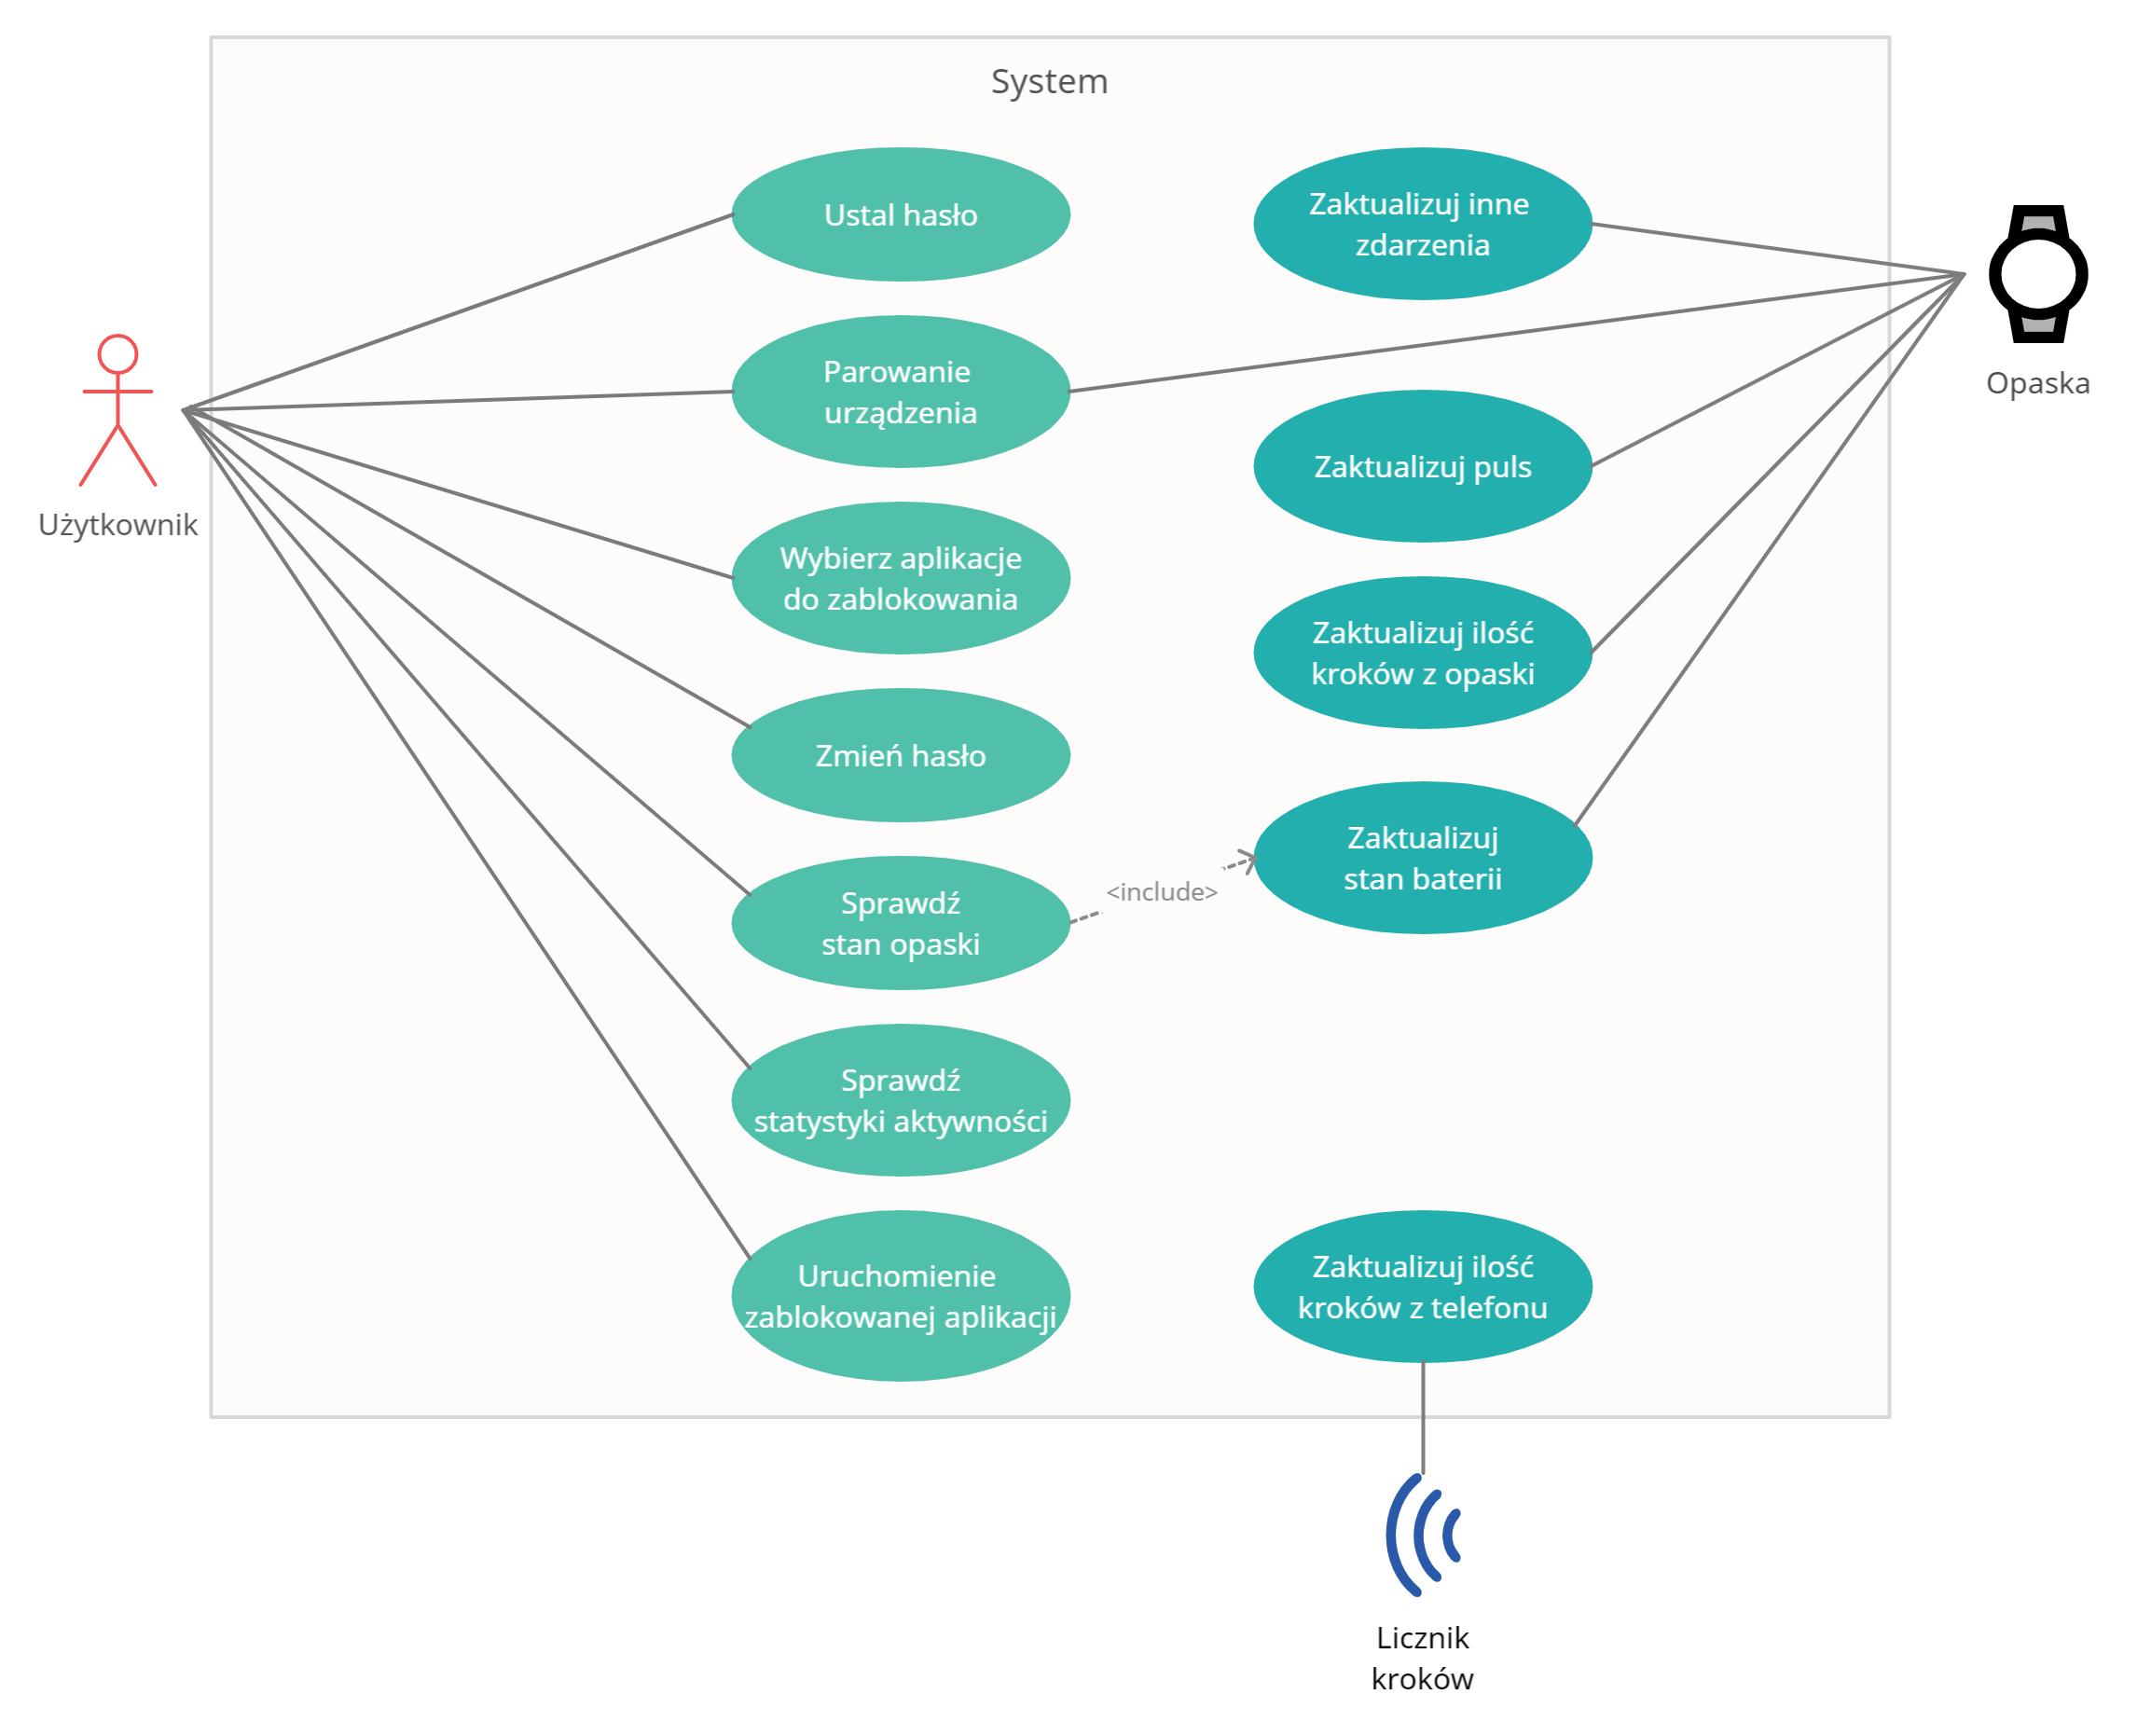
\includegraphics[width=0.9\textwidth]{UseCaseDiagram.png}
    \end{center}
    \caption{{\color{dgray}Diagram przypadków użycia w systemie.}} \label{use_case}
\end{figure}

\subsection{Ustal hasło}
W tym przypadku użytkownik aplikacji ustala hasło, które jest potrzebne przy odblokowywaniu dostępu do zablokowanych aplikacji. Aktorami są Użytkownik oraz System. Obecny przypadek użycia jest inicjowany przy pierwszym uruchomieniu aplikacji, kiedy nie istnieje jeszcze zaszyfrowany plik, w którym będzie przechowywane hasło. Po wykonaniu przypadku w systemie zostaje zarejestrowane hasło użytkownika, które będzie później wykorzystane w celu dezaktywacji blokady aplikacji. Scenariusz składa się z następującego przepływu głównego:
\begin{enumerate}
    \item Aplikacja wyświetla formularz zawierający pola Hasło oraz Powtórz hasło.
    \item Użytkownik wprowadza identyczne hasła do podanych pól oraz zatwierdza wprowadzone dane przyciskiem znajdującym się poniżej.
    \item System sprawdza zgodność haseł oraz czy spełniają wymagane kryteria.
    \item System tworzy zaszyfrowany plik i zapisuje w nim hasz hasła.
\end{enumerate}
Alternatywnie:
\newline\newline
\indent 3. Jeśli wprowadzone hasła nie są zgodne:
\begin{enumerate}[leftmargin=3\parindent]
    \item Zostaje wyświetlony komunikat o błędzie.
    \item Następuje powrót do kroku numer 2 w głównym przepływie.
\end{enumerate}

\subsection{Parowanie urządzenia}
W tym przypadku użytkownik aplikacji skanuje otoczenie, korzystając z modułu Bluetooth w poszukiwaniu najbliższej opaski MiBand, a następnie nawiązuje z nią pierwsze połączenie. Aktorami są Użytkownik, System oraz Opaska. Przypadek ten występuje przy pierwszym uruchomieniu systemu, kiedy zostało już ustalone hasło odblokowujące. Po zakończeniu system jest sparowany z opaską MiBand, z którą komunikacja jest kluczowym punktem działania systemu. W systemie zostaje także zapisany adres MAC opaski, dzięki czemu będzie można z łatwością ponownie połączyć się z nią. Główny przepływ składa się z następujących kroków:
\begin{enumerate}
    \item Użytkownik naciska przycisk ``Skan''.
    \item System rozpoczyna skanowanie urządzeń Bluetooth Low Energy w celu znalezienia Opaski.
    \item System wyświetla znalezione Opaski w formie listy. 
    \item Użytkownik wybiera Opaskę, do której się podłączy poprzez naciśnięcie na jej nazwę.
    \item System tworzy więź z wybraną Opaską i inicjuje pierwsze połączenie.
\end{enumerate}
Alternatywnie:
\newline\newline
\indent 3. Jeśli nie znaleziono żadnej Opaski:
\begin{enumerate}[leftmargin=3\parindent]
    \item Zostaje wyświetlony komunikat o błędzie.
    \item Następuje powrót do kroku numer 1 w głównym przepływie.
\end{enumerate}
\quad\newline
\indent 5. Jeśli wystąpi błąd połączenia z Opaską:
\begin{enumerate}[leftmargin=3\parindent]
    \item Następuje powrót do kroku numer 4 w głównym przepływie.
\end{enumerate}

\subsection{Wybierz aplikacje do zablokowania}
W tym przypadku użytkownik aplikacji wybiera z listy zainstalowanych aplikacji te, które będą blokowane przez system kiedy zostanie uruchomiona blokada. Aktorami są Użytkownik oraz System. Przypadek ten występuje, gdy istnieje plik z hasłem, opaska została sparowana, nie ma uruchomionej blokady oraz Użytkownik uruchomił aplikację. Po zakończeniu System posiada informację, na których aplikacjach uruchamiać blokadę. Główny przepływ składa się z następujących kroków:
\begin{enumerate}
    \item Użytkownik z poziomu głównego ekranu aplikacji przechodzi do Ustawień.
    \item Użytkownik wybiera opcję Zablokowane aplikacje.
    \item Użytkownik zaznacza aplikację z listy, którą chce zablokować bądź odblokować.
    \item System zapisuje aktualny stan aplikacji.
\end{enumerate}

\subsection{Zmień hasło}
W tym przypadku użytkownik aplikacji zmienia hasło odblokowujące dostęp do zablokowanych aplikacji. Aktorami są Użytkownik oraz System. Przypadek ten występuje, gdy istnieje plik z hasłem, opaska została sparowana, nie ma uruchomionej blokady oraz Użytkownik uruchomił aplikację. Po zakończeniu system posiada informację o nowym haśle, które będzie wykorzystywane od tej pory do odblokowywania dostępu. Główny przepływ składa się z następujących kroków:
\begin{enumerate}
    \item Użytkownik z poziomu głównego ekranu aplikacji przechodzi do Ustawień.
    \item Użytkownik wybiera opcję Zmień hasło.
    \item Użytkownik wpisuje odpowiednie wartości do pól Stare hasło, Nowe hasło oraz Powtórz nowe hasło oraz zatwierdza wprowadzone dane.
    \item System zapisuje hasz nowego hasła w zaszyfrowanym pliku.
\end{enumerate}
Alternatywnie: 
\newline\newline
\indent 3. Jeśli stare hasło jest błędne lub nowe hasło nie zgadza się z powtórzonym:
\begin{enumerate}[leftmargin=3\parindent]
    \item System wyświetla komunikat o błędnych wprowadzonych danych.
    \item Następuje powrót do kroku numer 3 w głównym przepływie.
\end{enumerate}
\quad\newline
\indent 4. Jeśli wystąpi błąd zapisu:
\begin{enumerate}[leftmargin=3\parindent]
    \item System wyświetla komunikat o błędzie zapisu.
    \item Następuje powrót do kroku numer 3 w głównym przepływie.
\end{enumerate}

\subsection{Sprawdź stan opaski}
W tym przypadku użytkownik aplikacji sprawdza podstawowe informacje na temat opaski oraz jej stan baterii.

\subsection{Sprawdź statystyki aktywności}

\subsection{Uruchomienie zablokowanej aplikacji}

\subsection{Zaktualizuj inne zdarzenia}

\subsection{Zaktualizuj puls}

\subsection{Zaktualizuj ilość kroków z opaski}

\subsection{Zaktualizuj stan baterii}

\subsection{Zaktualizuj ilość kroków z telefonu}

\section{Diagram komponentów}

W tej sekcji należy przedstawić diagramy komponentów dla odpowiednich elementów systemu zidentyfikowane na podstawie wcześniejszych rozważań

\section{Diagramy stanów}

W tej sekcji należy przedstawić diagramy stanów w których może znaleźć się system. Diagramy te są szczególnie istotne przy projektowaniu systemów czasu rzeczywistego.

\section{Projekt bazy danych}

W tej sekcji należy przedstawić projekt bazy danych. Należy omówić wycinek rzeczywistości i odpowiadające mu zidentyfikowane elementy systemu, których wartości będą podlegać utrwalaniu. Należy przedyskutować wybór typów danych dla atrybutów poszczególnych obiektów.  

\section{Opis protokołów}
\begin{itemize}
    \item inicjalizacja komunikacji z opaską
\end{itemize}

W projektowanym systemie główną rolę gra inteligentna opaska. Komunikuje się ona ze smartfonem przy użyciu technologii Bluetooth Low Energy oraz protokołu ATT. BLE w porównaniu
do klasycznego połączenia Bluetooth wykorzystuje znacznie niższe zasoby energii zachowując podobny zasięg, dzięki czemu znalazło
szerokie zastosowanie w urządzeniach peryferyjnych.
\subsection{Protokół ATT}
Protokół Attribute pozwala urządzeniom odczytywać i zapisywać drobne dane przechowywane na serwerze.
Przechowywane wartości są nazywane atrybutami. Atrybuty identyfikowane są poprzez
UUID, aby określić typ przechowywanych w nich danych. UUID mogą być powszechnie znanymi
numerami zdefiniowanymi w oficjalnej specyfikacji Bluetooth albo być
określone przez producenta jako 128-bitowa liczba. Wiadomości w tym
protokole są przesyłane przez kanały L2CAP, znanymi jako nośniki ATT. W ATT
występują dwie role: Klienta oraz Serwera. Urządzenie może pełnić obie te role
jednocześnie. Serwer przechowuje atrybuty oraz akceptuje żądania, komendy
oraz potwierdzenia pochodzące od klienta. Serwer wysyła także odpowiedzi na
żądania, a gdy zostanie skonfigurowany przez wyższą warstwę, wysyła asynchronicznie powiadomienia
do klienta, kiedy występują na nim określone zdarzenia.
\subsection{GATT}
Komunikacja aplikacji z opaską odbywa się przy wykorzystaniu GATT (Generic Attribute Profile). Jest to technologia zbudowana na protokole Attribute (ATT), która
ustala przebieg powszechnych operacji oraz framework dla danych transportowanych przez ATT.
GATT określa format danych przesyłanych przez protokół Attribute. Atrybuty są
formatowane jako Usługi oraz Charakterystyki. Usługi są zbiorem danych oraz
przypisanych im zachowań niezbędnych do zapewnienia określonej funkcji urządzenia.
Z kolei Charakterystyki są wartościami użytymi w Usłudze wraz z ich właściwościami
oraz informacjami o tym jak są wyświetlane bądź reprezentowane. Dzięki
wykorzystaniu określonej struktury danych przez GATT możliwe jest przeglądanie
dostępnych Usług oraz Charakterystyk, nawet gdy klient nie jest wyspecjalizowany
pod dany serwer.
\subsection{Komunikacja z MiBand 3}

	\cleardoublepage
	
	\chapter{Implementacja aplikacji}
\thispagestyle{chapterBeginStyle}
\label{rozdzial3}
W tym rozdziale określono szczegóły implementacyjne aplikacji. Scharakteryzowano wykorzystany język programowania oraz użyte biblioteki. Następnie opisano sposób uniemożliwienia dostępu do blokowanych aplikacji. W kolejnej sekcji opisano dokładnie protokół wykorzystywany do komunikacji z MiBandem 3 wraz z sekwencją autentykującą oraz konfiguracyjną. W ostatniej sekcji określono w jaki sposób aplikacja analizuje dane o aktywności użytkownika.

\section{Wykorzystane technologie}
Aplikacja została napisana przy użyciu języka \textbf{Kotlin} w wersji 1.4.31. Język ten, jest tworzony od 2011 roku przez Jetbrains z myślą, by zapewnić przemysłowo silny język obiektowy, który będzie lepszy od Javy ale wciąż będzie z nią w pełni interoperacyjny, aby umożliwić stopniową migrację istniejących już systemów. Głównymi zaletami korzystania z Kotlina w programowaniu na system Android jest zmniejszenie objętości kodu oraz możliwość wykorzystania funkcjonalności języka takich, jak korutyny, funkcje rozrzerzeń czy lambdy w istniejących bibliotekach Androida. Kod Kotlina jest także bardziej czytelny niż Javy, co prowadzi do zmniejszonej liczby błędów. 
\newline\newline
\indent Do implementacji bazy danych wykorzystano bibliotekę \textbf{Room}, tworzącą warstwę abstrakcji nad SQLite, by zapewnić płynny dostęp do bazy, zachowując pełną moc SQLite. Biblioteka ta pozwala między innymi zmniejszyć ilość powtarzalnego, skłonnego do generowania błędów kodu poprzez stosowanie anotacji oraz weryfikować zapytania SQL w czasie kompilacji. Aby zapewnić bezpieczeństwo bazy danych została ona zaszyfrowana przy użyciu biblioteki \textbf{SQLCipher}.
\newline\newline
\indent Do jeszcze większej optymalizacji kodu wykorzystano bibliotekę \textbf{Hilt}, która odpowiada za wstrzykiwanie zależności do klas. W przeciwieństwie do manualnego konstruowania klas wraz z ich zależnościami oraz wykorzystywaniu dodatkowych obiektów do zarządzania nimi, Hilt generuje je sam na podstawie określonych anotacji, a także zapewnia poprawne zarządzanie ich cyklem życia. Dzięki temu przy mniejszej ilości kodu można uzyskać lepszą wydajność w czasie działania aplikacji oraz zmiejszenie liczby błędów podczas kompilacji.
\newline\newline
\indent Do implementacji komunikacji z MiBandem została wykorzystana biblioteka \textbf{RxJava}, pozwalająca wykorzystać możliwości programowania reaktywnego, czyli paradygmatu programowania polegającego na przetwarzaniu strumieni danych i propagowaniu ich zmian, w aplikacjach na system Android. Przepływ danych pomiędzy aplikacją a opaską został opakowany w obiekty typu \textit{Observable}, co pozwoliło dokładnie monitorować stan wysyłanych danych oraz asynchronicznie oczekiwać odpowiedzi na poszczególne operacje.
\newline\newline
\indent Aby usprawnienić wydajność aplikacji wszystkie operacje zapisu do bazy danych oraz komunikacja z opaską są wykonywane w korutynach zoptymalizowanych pod operacje wejścia/wyjścia, dzięki czemu główny wątek aplikacji zostaje odciążony. Wykorzystano również \textbf{Data Binding}, aby uprościć odniesienia do elementów UI w kodzie aplikacji, co pozwala zwiększyć odporność na wycieki pamięci oraz wydajność. 

\section{Blokada dostępu do aplikacji}
Skuteczny sposób uniemożliwienia dostępu do aplikacji jest jedną z kluczowych części projektowanego systemu. Schemat blokady zaprezentowany w pracy opiera się na monitorowaniu aplikacji na pierwszym planie systemu Android. Aby dostać się do tych informacji wykorzystano usługę \textit{Usage Stats}, która zawiera statystyki korzystania z zainstalowanych aplikacji oraz zdarzenia takie, jak zablokowanie ekranu czy wyświetlenie aktywności danej aplikacji na ekranie. Proponowany system blokady pobiera zdarzenia z ostatnich 5 sekund, a następnie poszukuje w nich typu ``MOVE\_TO\_FOREGROUND''. Jeśli takie zdarzenie zostanie odnalezione, a aplikacja, która zainicjowała je, jest na liście aplikacji do zablokowania, następuje przejście do aktywności zawierającej pole do wpisania hasła. W przeciwnym razie system nie reaguje. Jeśli wprowadzone hasło było poprawne usługa blokująca zostaje zatrzymana i aplikacja nawiązuje próbę połączenia się z opaską. Poniżej przedstawiono zarys algorytmu blokującego w pseudokodzie.
\newline

\begin{algorithm}[H]
    \DontPrintSemicolon
    \SetAlgoLined
    \caption{Blokowanie dostępu do wybranych aplikacji} 
    \BlankLine
    \KwData{Lista zablokowanych aplikacji $BA$}
    \BlankLine
    \Begin{
        \While{blokada jest aktywna}{
            $events \gets $ zdarzenia z \textit{Usage Stats} z ostatnich 5 sekund \;
            \While{$events$.hasNext()}{
                $event \gets events$.next() \;
                \If{$event ==$ ``MOVE\_TO\_FOREGROUND'' $\land$ $event$.isIn($BA$)}{
                    Uruchom aktywność odpowiedzialną za wpisywanie hasła \;
                }
            }
            Poczekaj 5 sekund \;
        }
    }
\end{algorithm}

\section{Komunikacja z MiBand 3}
W projektowanym systemie główną rolę gra inteligentna opaska. Komunikuje się ona ze smartfonem przy użyciu Bluetooth Low Energy protokołem ATT korzystając z GATT. BLE w porównaniu do klasycznego połączenia Bluetooth wykorzystuje znacznie niższe zasoby energii zachowując podobny zasięg, dzięki czemu znalazło szerokie zastosowanie w urządzeniach peryferyjnych. W poniższych podrozdziałach opisano pokrótce pojęcia ATT i GATT oraz dokładnie przedstawiono zaimplementowany protokół komunikacji z opaską MiBand 3.
\subsection{ATT}
Protokół Attribute umożliwia urządzeniu, określonemu jako \textit{serwer}, odsłonić zbiór atrybutów i powiązanych z nimi wartości urządzeniu równorzędnemu, określonemu jako \textit{klient}. Atrybuty odsłonięte przez serwer mogą być odkryte, odczytane bądź nadpisane przez klienta, a także mogą być rozgłaszane przez serwer w ramach powiadomienia lub zasygnalizowania. Atrybut jest dyskretną wartością o trzech właściwościach powiązanych ze sobą:
\begin{itemize}
    \item typie,
    \item uchwycie,
    \item zestawie pozwoleń, które są zdefiniowane przez specyfikację wyższej warstwy wykorzystującą dany atrybut.
\end{itemize}
Typ atrybutu określa, co reprezentuje dany atrybut poprzez UUID (Universally Unique Identifier), ktore może zostać utworzone przez każdego, a następnie zostać opublikowane. Pozwala to rozpoznać atrybut niezależnie od nadanego mu przez serwer uchwytu. Uchwyt atrybutu jest unikalną, niezerową, 16-bitową wartością, która jednoznacznie identyfikuje dany atrybut w obrębie serwera, pozwalając klientowi odnieść się do niego podczas operacji odczytu oraz zapisu. Pozwolenia mogą być nadane atrybutowi w celu ograniczenia klientowi dostępu do zapisu lub odczytu.
\newline\newline
\indent Urządzenie może jednocześnie implementować zarówno rolę serwera jak i klienta oraz obie role mogą funkcjonować współbieżnie oraz komunikować się między sobą. Na każdym urządzeniu Bluetooth może znajdować się maksymalnie jedna instancja serwera.
\newline\newline
\indent Wszystkie prośby protokołu Attribute są przesyłane poprzez \textit{nosiciela ATT}. Między urządzeniami może być wielu nosicieli, gdzie każdy z nich korzysta z osobnego kanału L2CAP oraz może mieć inną konfigurację. W przypadku BLE, wykorzystywany jest pojedynczy nosiciel ATT, który używa stałego kanału dostępnego od ustanowienia połączenia ACL. Można jednak skonfigurować dodatkowych nosicieli używając L2CAP. Więcej informacji na temat protokołu ATT można znaleźć w \cite{BT-Corev5.2}. 

\subsection{GATT}
Profil Generic Attribute (GATT) definiuje framework wykorzystujący protokół Attribute, określający procedury i formaty danych znajdujących się wewnątrz profilu. Zdefiniowane procedury obejmują odkrywanie, odczyt, zapis, powiadamianie oraz sygnalizację. Profil ten został zaprojektowany do wykorzystania przez aplikacje bądź inny profil, aby umożliwić klientowi komunikację z serwerem poprzez opakowanie protokołu ATT w bardziej przystępną formę.
\newline\newline
\indent Profil GATT określa strukturę, w której odbywa się wymiana danych. Najwyższym poziomem jest profil zawierający liczne \textit{usługi} będące zbiorem danych oraz przypisanych im zachowań niezbędnych do zapewnienia określonej funkcji. Usługi składają się z \textit{charakterystyk}, z których każda zawiera określoną wartość oraz opcjonalne informacje na jej temat. Usługi oraz charakterystyki wraz ze swoimi komponentami zawierają dane profilu, które są przechowywane w Atrybutach na serwerze. Dzięki wykorzystaniu określonej struktury danych przez GATT możliwe jest przeglądanie dostępnych Usług oraz Charakterystyk, nawet gdy klient nie jest wyspecjalizowany pod dany serwer. Więcej informacji na temat GATT można znaleźć w \cite{BT-Corev5.2}.

\subsection{Wykorzystane usługi i charakterystyki}
Do uzyskania potrzebnych danych z opaski zostały użyte poniżej opisane usługi. Dla każdej z nich przedstawiono listę wykorzystanych charakterystyk z krótkim opisem, za co odpowiadają. Poniższe wartości zostały zidentyfikowane na podstawie przechwytywania pakietów ATT komunikacji MiBanda 3 z aplikacją Gadgetbridge \cite{Gadgetbridge} przy użyciu open-sourcowego sniffera Wireshark \cite{Wireshark} oraz analizie kodu źródłowego Gadgetbridge.

\subsubsection{Usługa 0000fee0-0000-1000-8000-00805f9b34fb}
Jest to usługa odpowiadająca w głównej mierze za podstawowe funkcjonalności opaski MiBand 3. Pozwala zmodyfikować ustawienia urządzenia, zapisać informacje o użytkowniku oraz odczytać dane o stanie baterii i aktywności użytkownika. Jest to najczęściej wykorzystywana usługa w aplikacji.

\begin{table}[H]
    \bgroup
    \def\arraystretch{1.5}%
    \begin{tabular}{|ll|}
    \hline
    \textbf{Charakterystyka}                      & \textbf{Opis}                                                                                                                \\ \hline
    \textbf{00000003-0000-3512-2118-0009af100700} & \begin{tabular}[c]{@{}l@{}}Charakterystyka pozwalająca na konfigurację ustawień \\ opaski.\end{tabular}                      \\
    \textbf{00000006-0000-3512-2118-0009af100700} & \begin{tabular}[c]{@{}l@{}}Charakterystyka zawierająca informacje o stanie baterii \\ opaski.\end{tabular}                   \\
    \textbf{00000007-0000-3512-2118-0009af100700} & \begin{tabular}[c]{@{}l@{}}Charakterystyka przechowująca liczbę wykonanych kroków \\ danego dnia.\end{tabular}               \\
    \textbf{00000008-0000-3512-2118-0009af100700} & Charakterystyka zawierająca dane użytkownika.                                                                                \\
    \textbf{00000010-0000-3512-2118-0009af100700} & \begin{tabular}[c]{@{}l@{}}Charakterystyka zawierająca informacje na temat zdarzeń \\ wykrywanych przez opaskę.\end{tabular} \\
    \textbf{00002a2b-0000-1000-8000-00805f9b34fb} & Charakterystyka przechowująca aktualną datę i godzinę,                                                                       \\ \hline
    \end{tabular}
    \egroup
    \caption{{\color{dgray}Wykorzystane charakterystyki z usługi 0000fee0-0000-1000-8000-00805f9b34fb.}} \label{miliservice}
\end{table}

\subsubsection{Usługa 0000fee1-0000-1000-8000-00805f9b34fb}
Jest to usługa zawierająca przede wszystkim charakterystykę wykorzystywaną w procesie autentykacji połączenia oraz parowania. W usłudze tej znajduje się też sporo niezidentyfikowanych charakterystyk, które nie są wymagane do działania aplikacji. Dlatego więc zostały pominięte.
\begin{table}[H]
    \bgroup
    \def\arraystretch{1.5}%
    \begin{tabular}{|ll|}
    \hline
    \textbf{Charakterystyka}                      & \textbf{Opis}                                                                                                                \\ \hline
    \textbf{00000009-0000-3512-2118-0009af100700} & \begin{tabular}[c]{@{}l@{}}Charakterystyka wykorzystywana do autentykacji  \\ połączenia między opaską a klientem\end{tabular} \\ \hline
    \end{tabular}
    \egroup
    \caption{{\color{dgray}Wykorzystane charakterystyki z usługi 0000fee1-0000-1000-8000-00805f9b34fb.}} \label{miband2service}
\end{table}

\subsubsection{Usługa 0000180d-0000-1000-8000-00805f9b34fb}
Jest to usługa zdefiniowana przez Bluetooth Special Interest Group odpowiadająca za komunikację między sensorem akcji serca a innym klientem GATT. Za jej pomocą można uzyskać informację o pulsie użytkownika oraz skonfigurować automatyczne pomiary. 

\begin{table}[H]
    \bgroup
    \def\arraystretch{1.5}%
    \begin{tabular}{|ll|}
    \hline
    \textbf{Charakterystyka}                      & \textbf{Opis}                                                                                                              \\ \hline
    \textbf{00002a37-0000-1000-8000-00805f9b34fb} & \begin{tabular}[c]{@{}l@{}}Charakterystyka wykorzystywana do odczytu aktualnej \\ wartości pulsu użytkownika.\end{tabular} \\
    \textbf{00002a39-0000-1000-8000-00805f9b34fb} & \begin{tabular}[c]{@{}l@{}}Charakterystyka odpowiedzialna za konfigurację sensora \\ akcji serca w opasce.\end{tabular}    \\ \hline
    \end{tabular}
    \egroup
    \caption{{\color{dgray}Wykorzystane charakterystyki z usługi 0000180d-0000-1000-8000-00805f9b34fb.}} \label{heartrateservice}
\end{table}

\subsubsection{Usługa 0000180a-0000-1000-8000-00805f9b34fb}
Jest to usługa również zdefiniowana przez Bluetooth Special Interest Group. Odpowiada za dostarczenie informacji o urządzeniu. W tym wypadku jest to informacja o numerze seryjnym opaski oraz wersjach sprzętu i oprogramowania.

\begin{table}[H]
    \bgroup
    \def\arraystretch{1.5}%
    \begin{tabular}{|ll|}
    \hline
    \textbf{Charakterystyka}                      & \textbf{Opis}                                                                                                      \\ \hline
    \textbf{00002a25-0000-1000-8000-00805f9b34fb} & \begin{tabular}[c]{@{}l@{}}Charakterystyka wykorzystywana do odczytu numeru \\ seryjnego opaski.\end{tabular}      \\
    \textbf{00002a27-0000-1000-8000-00805f9b34fb} & \begin{tabular}[c]{@{}l@{}}Charakterystyka wykorzystywana do odczytu wersji \\ sprzętowej opaski.\end{tabular}        \\
    \textbf{00002a28-0000-1000-8000-00805f9b34fb} & \begin{tabular}[c]{@{}l@{}}Charakterystyka wykorzystywana do odczytu wersji \\ oprogramowania opaski.\end{tabular} \\ \hline
    \end{tabular}
    \egroup
    \caption{{\color{dgray}Wykorzystane charakterystyki z usługi 0000180a-0000-1000-8000-00805f9b34fb.}} \label{deviceservice}
\end{table}

\subsection{Autentykacja połączenia}
Aby konfigurować oraz odczytywać informacje o aktywności z MiBanda wymagana jest prosta autoryzacja. W przeciwnym razie ma dostępu do większości charakterystyk urządzenia, a połączenie zostanie zerwane po 30 sekundach. Sekwencja autentykacyjna wygląda w następujący sposób. Najpierw do opaski należy wysłać klucz, który zostanie wykorzystany do autentykacji połączenia. Wykonuje się to przy pierwszym połączeniu z urządzeniem. Następnie wysyłana jest prośba do MiBanda o podanie losowej liczby. Po jej otrzymaniu należy zaszyfrować ją algorytmem AES korzystając z klucza podanego przy parowaniu opaski, odesłać i przesłać aktualną datę do odpowiedniej charakterystyki. Po otrzymaniu potwierdzenia połączenie jest zatwierdzone i można przejść do sekwencji konfigurującej. Aktualna data przesyłana jest jako tablica bajtów, gdzie wartości to: rok $\land$ 0xff, (rok $\gg$ 8) $\land$ 0xff, miesiąc $\land$ 0xff, dzień miesiąca $\land$ 0xff, godzina $\land$ 0xff, minuty $\land$ 0xff, sekundy $\land$ 0xff, dzień tygodnia $\land$ 0xff oraz 0.
\newline

\begin{algorithm}[H]
    \DontPrintSemicolon
    \SetAlgoLined
    \caption{Parowanie z MiBandem 3} 
    \BlankLine
    \KwData{Tablica bajtów zawierająca klucz wykorzystywany do szyfrowania $K$, Zmienna logiczna $pair$ mówiąca, czy urządzenie jest sparowane}
    \BlankLine
    \Begin{
        $authorisationChar \gets 00000009-0000-3512-2118-0009af100700$\;
        Włącz powiadomienia na $authorisationChar$\;
        \If{$pair$}{
            Wyślij do $authorisationChar \longrightarrow ByteArray(0x01, 0x00) + K $\;
            \If{Otrzymano $odpowiedz \gets ByteArray(0x10, 0x01, 0x01)$}{
                Przejdź do autentykacji \;
            }
        }
    }
\end{algorithm}
\quad\newline\newline
\begin{algorithm}[H]
    \DontPrintSemicolon
    \SetAlgoLined
    \caption{Autentykacja z MiBandem 3} 
    \BlankLine
    \KwData{Tablica bajtów zawierająca klucz wykorzystywany do szyfrowania $K$}
    \BlankLine
    \Begin{
        $authorisationChar \gets 00000009-0000-3512-2118-0009af100700$\;
        $timeChar \gets 00002a2b-0000-1000-8000-00805f9b34fb$\;
        Włącz powiadomienia na $authorisationChar$\;
        Wyślij do $authorisationChar \longrightarrow ByteArray(0x02, 0x00)$\;
        \If{Otrzymano $odpowiedz \gets ByteArray(0x10, 0x02, 0x01, \dots)$}{
            $numToEncrypt \gets odpowiedz \left[ 3:19 \right]$ \;
            Wyślij do $authorisationChar \longrightarrow ByteArray(0x03, 0x00) + AES(K, numToEncrypt)$ \;
            Wyślij do $timeChar$ aktualną datę\;
        }
        \If{Otrzymano $odpowiedz \gets ByteArray(0x10, 0x03, 0x01, \dots)$}{
            Przejdź do konfiguracji\;
        }
    }
\end{algorithm}

\subsection{Sekwencja konfigurująca}
Po udanej autoryzacji połączenia należy skonfigurować działanie opaski. Odbywa się to za pomocą sekwencji operacji zapisu, głównie do charakterystyki o UUID równym ``00000003-0000-3512-2118-0009af100700'' oraz włączeniu powiadamiania na odpowiednich charakterystykach. Po skonfigurowaniu urządzenie będzie automatycznie przesyłać odpowiednie dane o aktywności w najmniejszych możliwych odstępach czasu. Czynności konfiguracyjne zostały zidentyfikowane na podstawie porównania przechwyconych pakietów ATT z kodem źródłowym Gadgetbridge. Poniżej opisano szerzej niektóre z wysyłanych danych, które były zbyt obszerne, aby przedstawić je w pseudokodzie. 
\newline\newline
\indent Format daty jest przestawiony jako tablica bajtów, zawierająca każdy znak z ``dd/MM/yyyy'' skonwertowany na bajt. Wartość celu fitness obliczana jest jako dwuelementowa tablica bajtów, gdzie wartości to wartość celu $\land$ 0xff oraz (wartość celu $\gg$ 8) $\land$ 0xff. Dane użytkownika są formatowane do wysłania jako tablica bajtów zawierająca: 0x4f, 0x00, 0x00, rokUrodzenia $\land$ 0xff, (rokUrodzenia $\gg$ 8)$\land$ 0xff, miesiąc, dzien, płeć (0x00 lub 0x01), wzrost $\land$ 0xff, (wzrost $\gg$ 8) $\land$ 0xff, waga $\times$ 200 $\land$ 0xff, (waga $\times$ 200 $\gg$ 8) $\land$ 0xff, id $\land$ 0xff, (id $\gg$ 8) $\land$ 0xff, (id $\gg$ 16) $\land$ 0xff oraz (id $\gg$ 24) $\land$ 0xff.
\newline\newline
\begin{algorithm}[H]
    \DontPrintSemicolon
    \SetAlgoLined
    \caption{Konfiguracja MiBanda 3 - Część 1} 
    \BlankLine
    \Begin{
        $settingsChar \gets 00000003-0000-3512-2118-0009af100700$\;
        $batteryChar \gets 00000006-0000-3512-2118-0009af100700$\;
        $eventsChar \gets 00000010-0000-3512-2118-0009af100700$\;
        $userChar \gets 00000008-0000-3512-2118-0009af100700$\;
        $hrControlChar \gets 00002a39-0000-1000-8000-00805f9b34fb$\;
        $hrChar \gets 00002a37-0000-1000-8000-00805f9b34fb$\;
        $stepsChar \gets 00000007-0000-3512-2118-0009af100700$\;
        $serialNumChar \gets 00002a25-0000-1000-8000-00805f9b34fb$\;
        $hardwareChar \gets 00002a27-0000-1000-8000-00805f9b34fb$\;
        $softwareChar \gets 00002a28-0000-1000-8000-00805f9b34fb$\;
        \;
        Włącz powiadomienia na $settingsChar, batteryChar$ oraz $eventsChar$\;
        Odczytaj wartość z $serialNumChar, hardwareChar, softwareChar$ oraz $batteryChar$\;
        Ustaw język angielski wysyłając $ByteArray(0x06, 0x17, 0x00, 0x65, 0x6e, 0x5f, 0x55, 0x53)$ do $settingsChar$ \;
        Wyłącz odblokowywanie ekranu w opasce wysyłając $ByteArray(0x06, 0x16, 0x00, 0x00)$ do $settingsChar$\;
        Wyłącz tryb nocny wysyłając $ByteArray(0x1a, 0x00)$ do $settingsChar$\;
        Ustaw format daty wysyłając $ByteArray(0x06, 0x1e, 0x00)+ format$ do $settingsChar$, gdzie $format$ to opisany powyżej przetworzony łańcuch znaków\;
        Ustaw format wyświetlanej daty wysyłając $ByteArray(0x06, 0x0a, 0x00, 0x03)$ do $settingsChar$\;
        Ustaw 24-godzinny zegar wysyłając $ByteArray(0x06, 0x02, 0x00, 0x01)$ do $settingsChar$\;
        Ustaw przykładowe dane o użytkowniku wysyłając $userInfo$ do $settingsChar$, gdzie $userInfo$ to przetworzone dane o użytkowniku opisane powyżej\;
        Ustaw jednostki metryczne wysyłając $ByteArray(0x06, 0x03, 0x00, 0x00)$ do $settingsChar$\;
        Włącz powiadomienia na $userChar$\;
        Ustaw lokalizację noszenia opaski na lewą rękę wysyłając $ByteArray(0x20, 0x00, 0x00, 0x02)$ do $userChar$\;
        Ustaw cel fitness wysyłając $ByteArray(0x10, 0x00, 0x00, x[0], x[1], 0x00, 0x00)$ do $userChar$, gdzie $x$ to przetworzona wartość celu\;
        Ustaw elementy menu opaski wysyłając $ByteArray(0x0a, 0x7f, 0x30, 0x00, 0x01, 0x02, 0x03, 0x04, 0x05, 0x06, 0x07, 0x08)$ do $settingsChar$\;
        Wyłącz w opasce tryb ``Nie przeszkadzać'' wysyłając $ByteArray(0x09, 0x82)$ do $settingsChar$\;
        Wyłącz gest obrotu nadgarstka do zmiany pozycji w menu wysyłając $ByteArray(0x06, 0x0d, 0x00, 0x00)$ do $settingsChar$\;
        Wyłącz gest podniesienia nadgarstka do włączenia ekranu opaski wysyłając $ByteArray(0x06, 0x05, 0x00, 0x00)$ do $settingsChar$\;
        Włącz wyświetlanie ID dzwoniącego w opasce wysyłając $ByteArray(0x06, 0x10, 0x00, 0x00, 0x01)$ do $settingsChar$\;
        Wyłącz powiadomienia o celu fitness wysyłając $ByteArray(0x06, 0x06, 0x00, 0x00)$ do $settingsChar$\;
        Wyłącz powiadomienia o nieaktywności wysyłając $ByteArray(0x08, 0x00, 0x3c, 0x00, 0x04, 0x00, 0x15, 0x00, 0x00, 0x00, 0x00, 0x00)$ do $settingsChar$\;
        Włącz wspomaganie detekcji snu przez pomiar pulsu wysyłając $ByteArray(0x15, 0x00, 0x01)$ do $hrControlChar$\;
    }
\end{algorithm}
\quad\newline\newline
\begin{algorithm}[H]
    \DontPrintSemicolon
    \SetAlgoLined
    \caption{Konfiguracja MiBanda 3 - Część 2} 
    \BlankLine
    \Begin{
        Włącz powiadomienie o utracie połączenia wysyłając $ByteArray(0x06, 0x0c, 0x00, 0x01, 0x00, 0x00, 0x00, 0x00)$ do $settingsChar$\;
        Włącz powiadomienie o nawiązaniu połączenia wysyłając $ByteArray(0x06, 0x01, 0x00, 0x01)$ do $settingsChar$\;
        Ustaw interwał automatycznego pomiaru pulsu na minimalny wysyłając $ByteArray(0x14, 0x01)$  do $hrControlChar$\;
        Poproś o alarmy wysyłając $0x0d$ do $settingsChar$\;
        Włącz powiadomienia na $hrChar$ oraz $stepsChar$\;
    }
\end{algorithm}

\section{Analiza rejestrowanych danych o aktywności}
Aby proponowany system działał poprawnie niezbędna jest analiza gromadzonych przez opaskę oraz sensor kroków danych. Aplikacja rozróżnia 4 typy aktywności:
\begin{itemize}
    \item puls,
    \item kroki rejestrowane w opasce,
    \item kroki rejestrowane w telefonie,
    \item oraz inne zdarzenia.
\end{itemize}
Próbki pulsu oraz kroków są przechowywane w bazie danych w celu analizy. Natomiast wykrycie zdarzeń innego typu samo w sobie jest przesłanką do zablokowania systemu, więc nie ma potrzeby ich przechowywania. W poniższych akapitach opisano sposoby monitorowania zarejestrowanych próbek i zdarzeń oraz sytuacje, w których jest uruchamiana blokada.
\newline\newline
\indent Dane o akcji serca są analizowane w następujący sposób. Każda nadchodząca próbka z pomiarem równym 0 oraz brak zarejestrowania żadnej próbki w ciągu 90 sekund, świadczy o tym, że opaska została zdjęta i jest to przesłanka do blokady systemu. Z testów przeprowadzonych podczas rozwoju aplikacji wynikło, że monitorowanie tych czynników z wykorzystaniem podanych wartości jest ważne dla poprawnego określenia, czy opaska znajduje się na ręce, gdyż MiBand 3 rejestruje zdarzenia z opóźnieniem, więc odpowiednie zdarzenie o zdjęciu opaski nadchodziło po kilku minutach, co nie zapewnia wystarczającego bezpieczeństwa. Z kolei łączenie z opaską również jest obarczone sporym opóźnieniem, dlatego czasem w ciągu 60 sekund (najkrótszy możliwy okres pomiędzy automatycznymi pomiarami pulsu) od włączenia systemu monitorującego nie rejestrowano żadnej próbki pulsu. Z tego powodu okres pomiędzy pobieraniem próbek z bazy musiał zostać zwiększony do 90 sekund.
\newline\newline
\indent Dane o krokach są analizowane na podstawie różnic w tempie wzrostu między próbkami z opaski oraz smartfona. Co 90 sekund system pobiera próbki z ostatnich 90 sekund. Jeśli dla jednego ze źródeł nie zarejestrowano nowych próbek, system pobiera datę ostatniego pomiaru z tego źródła, a następnie dopisuje do listy próbek z drugiego źródła próbki starsze niż 90 sekund i młodsze od ostatniej próbki z pierwszego źródła. Krok ten został podjęty w celu wykrycia sytuacji, gdzie tylko jedno urządzenie porusza się, jednak na tyle wolno, że system myślałby, że tempa wzrostu pomiędzy tymi źródłami są akceptowalne. Tempo wzrostu jest określone jako amplituda wartości kroków z pobranych wcześniej próbek, biorąc poprawkę na możliwość pobrania próbek z okresu, gdy zmienia się data, co powoduje rozpoczęcie liczenia kroków od 0. Akceptowalna wartość amplitudy wynosi $\leq 30$. Jest to uwarunkowane tym, że przy niższych wartościach system mógłby aktywować się przy poruszaniu się wraz z telefonem, a przy wyższych system nie zareagowałby w wystarczającym stopniu na podejrzane sytuacje.
\newline\newline
\indent Oprócz analizy próbek aktywności system reaguje też na wykrywane zdarzenia. System rejestruje zdjęcie opaski, zaśnięcie oraz utratę połączenia. W przypadku dwóch pierwszych sytuacji, blokada jest uruchamiana natychmiastowo. Natomiast w przypadku utraty połączenia podejmowane są dwie próby ponownego połączenia. Jeśli nie uda się nawiązać ponownie połączenia uruchamiana jest blokada.
	\cleardoublepage
	
	\chapter{Instrukcja obsługi}
\thispagestyle{chapterBeginStyle}
\label{rozdzial4}

W tym rozdziale omówiono wymagania wobec środowiska, w którym będzie instalowana będzie opisana w pracy aplikacja. Przedstawiono procedurę instalacji oraz jak przeprowadzić podstawową konfigurację. W następnej sekcji przedstawiono kilka przykładów użycia aplikacji.

\section{Instalacja i konfiguracja}
\subsection{Wymagania sprzętowe}
Aplikacja została stworzona pod system Android Pie. Do działania jest wymagany moduł Bluetooth w wersji co najmniej 4.0 oraz posiadanie smartbanda MiBand 3. Do zainstalowania aplikacji potrzeba minimalnie około 23 MB wolnego miejsca. 
\subsection{Instalacja}
Aplikację można zainstalować przy użyciu dołączonego do pracy pliku \textit{lockband.apk}. Aby umożliwić instalowanie aplikacji z plików APK należy nadać odpowiedniej aplikacji (w tym przypadku menadżerowi plików) pozwolenie na instalowanie nieznanych aplikacji. Lokalizacja tego ustawienia może się znacząco różnić w zależności od wersji nakładki systemowej. Następnie należy pobrać plik APK na smartfona. W kolejnym kroku należy znaleźć pobrany wcześniej plik korzystając z menedżera plików. Ostatnim krokiem jest stuknięcie w plik APK, by uruchomić instalację.
\subsection{Pierwsze uruchomienie}
Podczas pierwszego uruchomienia aplikacja na początku prosi o udzielenie potrzebnych pozwoleń: Lokalizacji, potrzebnej do korzystania z Bluetooth oraz Dostępu do danych o użyciu, koniecznych do monitorowania wyświetlanych aplikacji. Użytkownik zostaje przekierowany do ustawień, gdzie może udzielić pozwolenia na wykorzystanie danych o użyciu. Następnie użytkownik może powrócić do aplikacji, gdzie zostanie wyświetlony monit o udzielenie pozwolenia na dostęp do lokalizacji. 
\begin{figure}[H]
    \begin{center}
        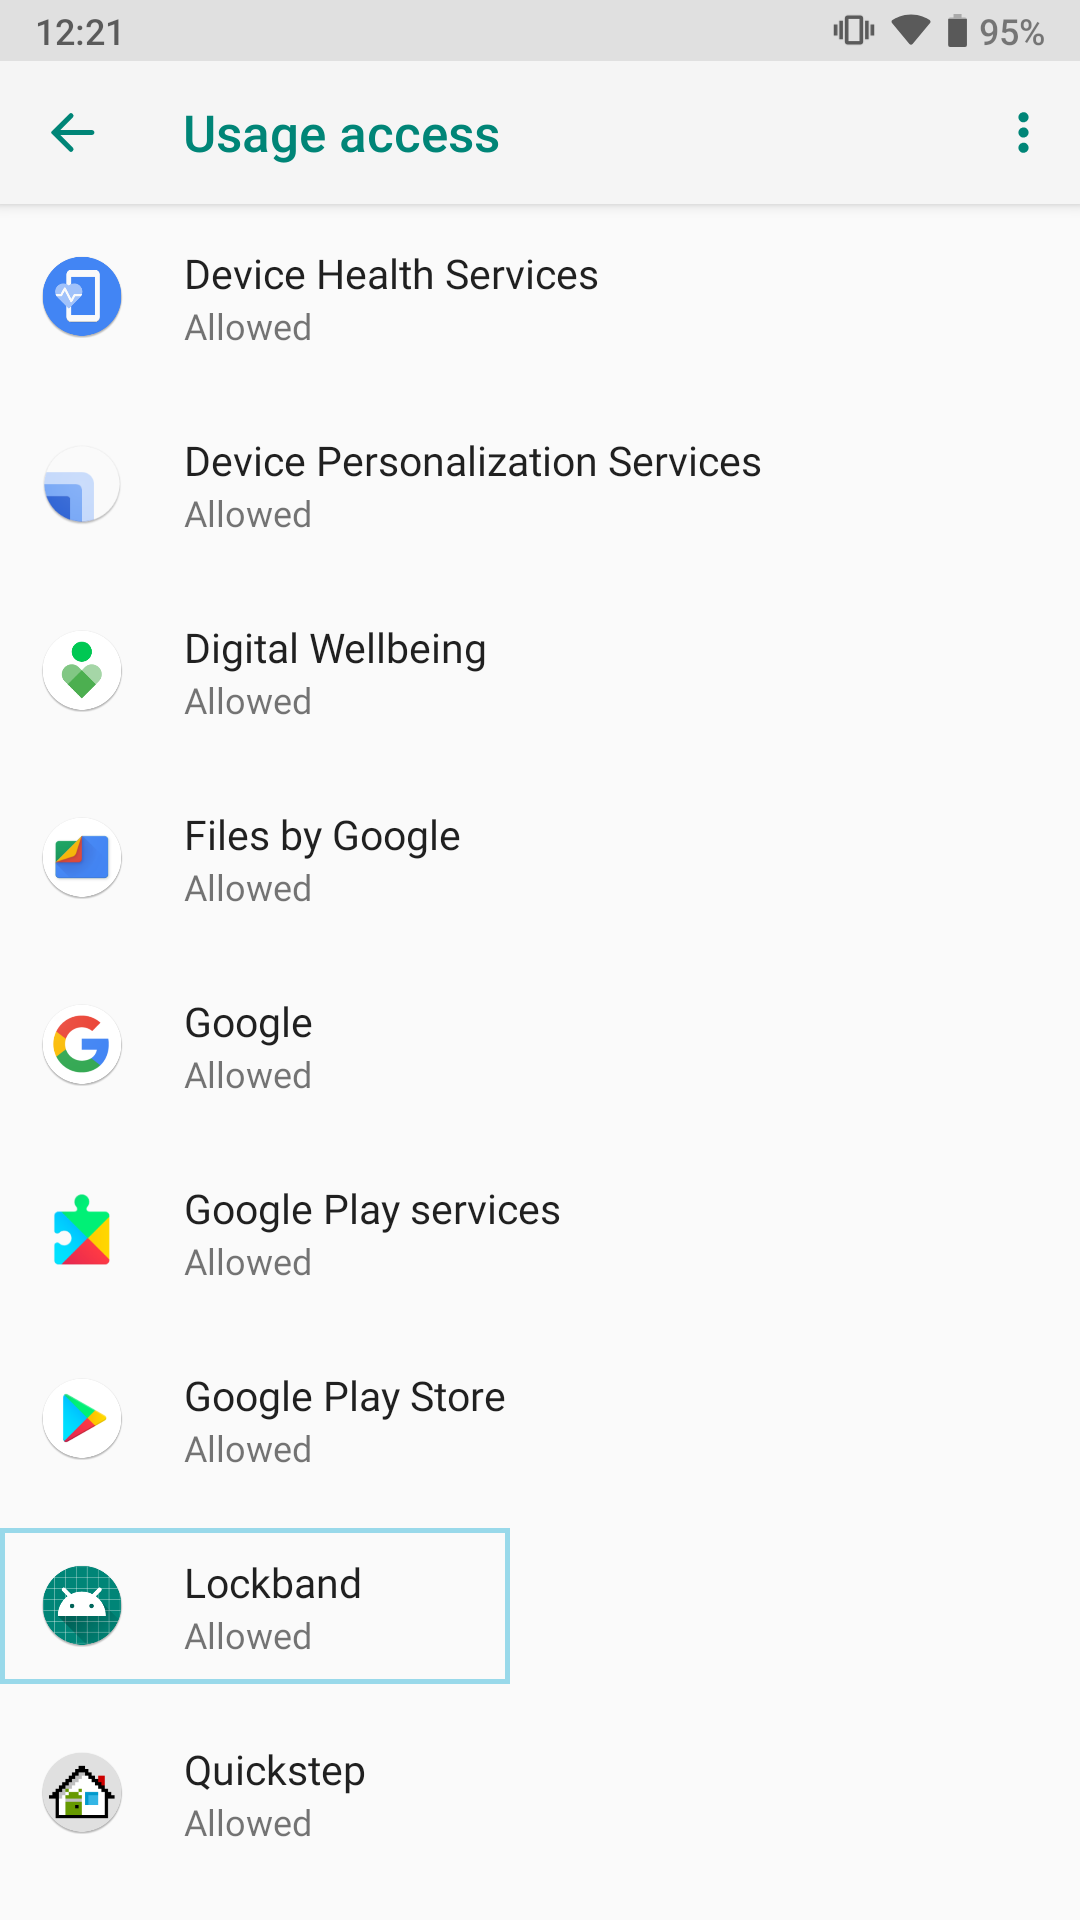
\includegraphics[width=0.27\textwidth]{app_screenshots/usage_stats_permission.png}
        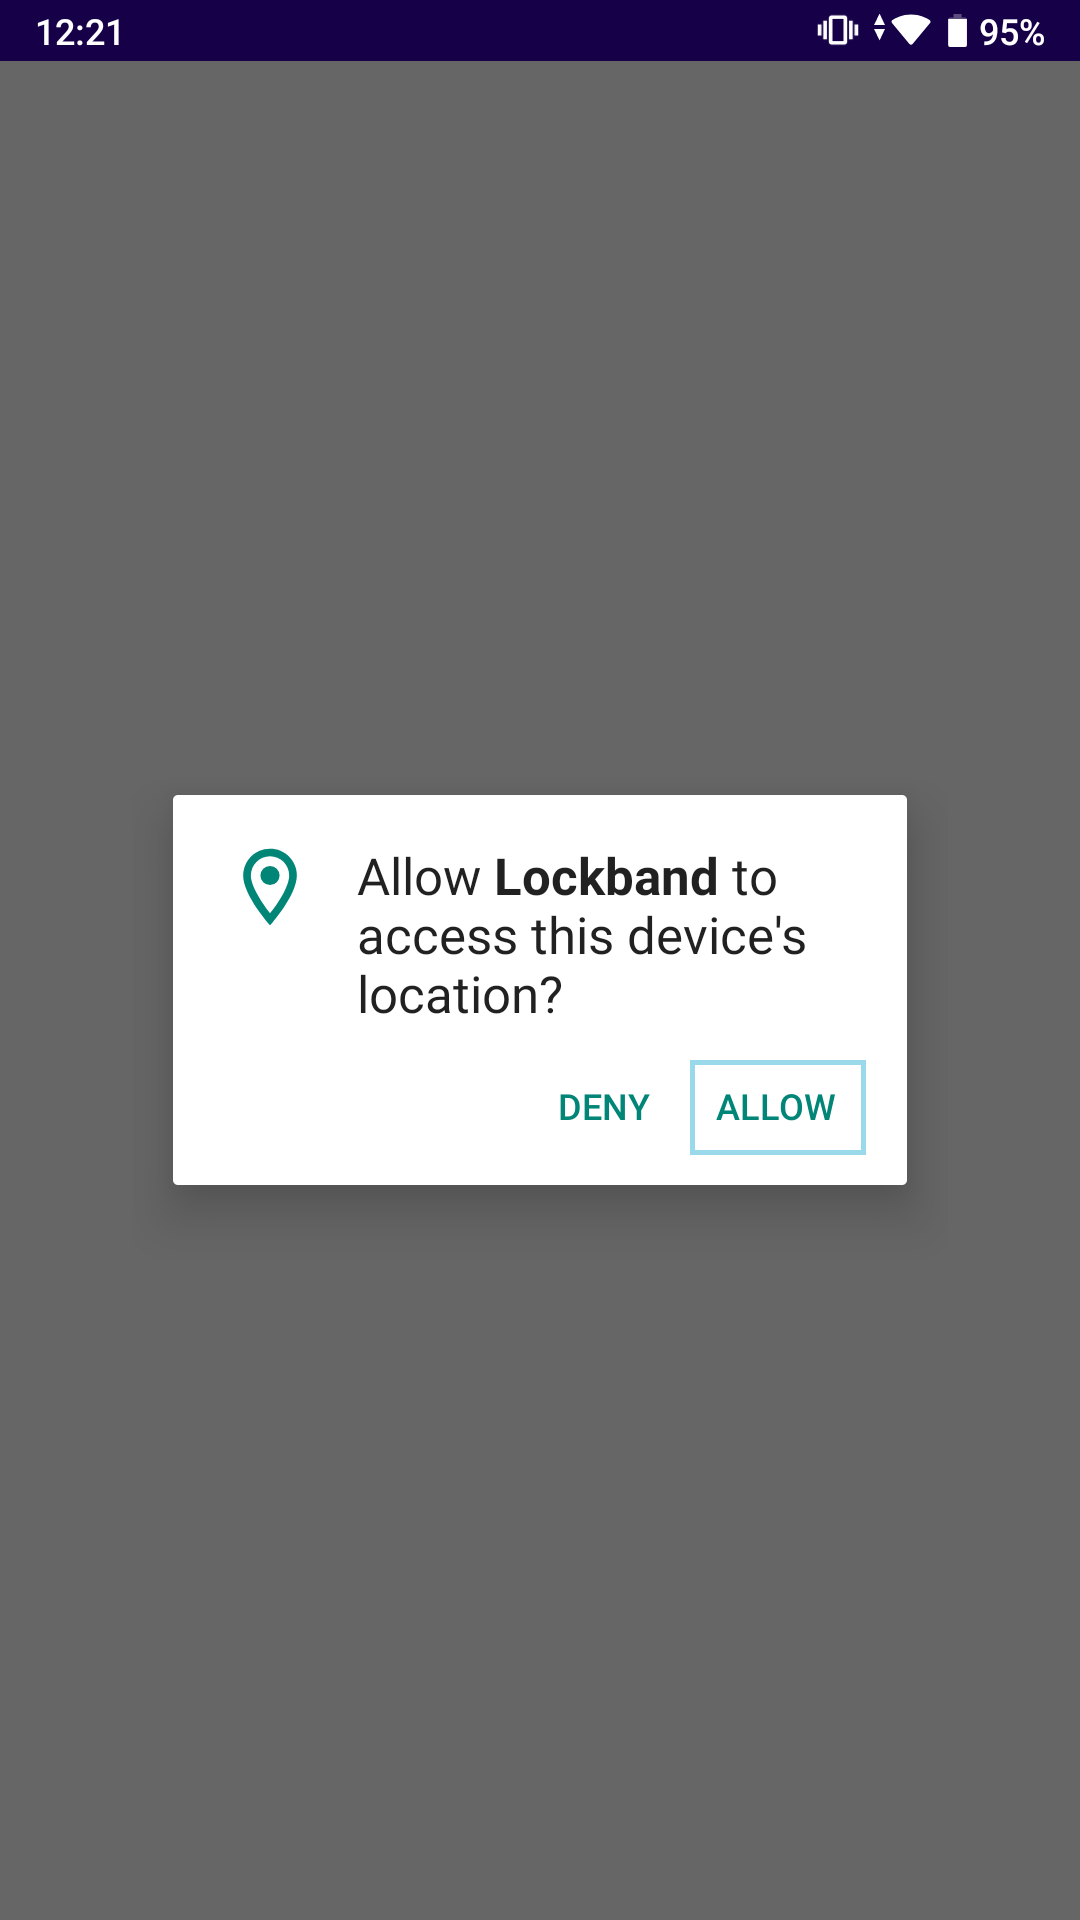
\includegraphics[width=0.27\textwidth]{app_screenshots/location_permission.png}
    \end{center}
    \caption{{\color{dgray}Udzielanie pozwoleń aplikacji.}} \label{usageStats}
\end{figure}
Kolejnym etapem konfiguracji jest ustalenie hasła, które zostanie wykorzystane do odblokowania dostępu do chronionych aplikacji. Użytkownikowi zostaje wyświetlony formularz, w którym należy wprowadzić dwa identyczne hasła, a następnie zatwierdzić je przyciskiem poniżej. Wygląd formularza można zobaczyć w poniższej grafice.
\begin{figure}[H]
    \begin{center}
        \setlength{\fboxsep}{0pt}%
        \setlength{\fboxrule}{0.27pt}%
        \fbox{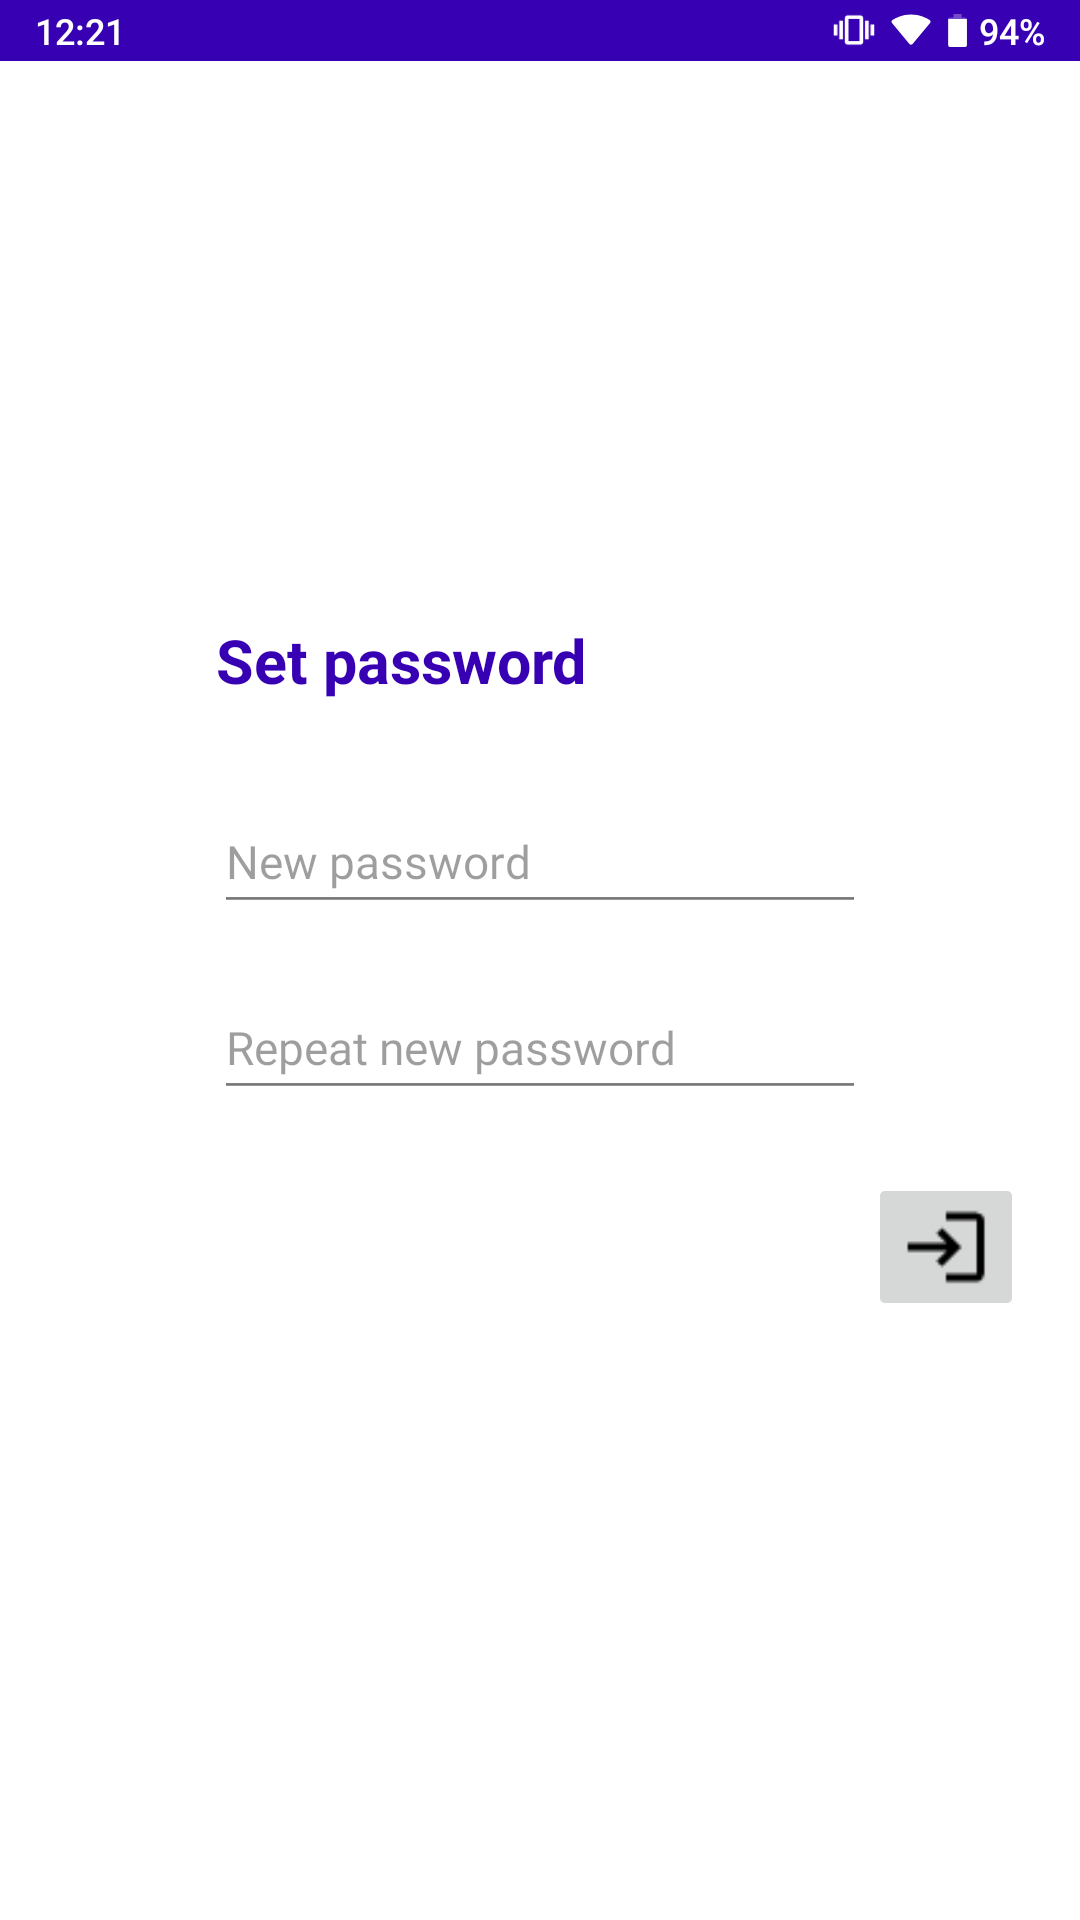
\includegraphics[width=0.3\textwidth]{app_screenshots/set_password.png}}
    \end{center}
    \caption{{\color{dgray}Formularz kreacji hasła.}} \label{setPassword}
\end{figure}
Ostatnim etapem konfiguracji jest sparowanie opaski MiBand 3 z aplikacją. W tym celu zostaje wyświetlona aktywność odpowiedzialna za skanowanie pobliskich urządzeń Bluetooth. Po naciśnięciu przycisku \textit{Scan for devices} zostaje uruchomione skanowanie z nałożonym filtrem na typ urządzenia. Jeśli za pierwszym razem opaska nie zostanie znaleziona należy powtórzyć skan. Po znalezieniu urządzenia zostaje ono wyświetlone na liście. Aby rozpocząć proces parowania należy nacisnąć nazwę danego urządzenia. Po zakończeniu parowania konfiguracja dobiega końca i użytkownik zostaje przeniesiony do głównego menu aplikacji. Inne sprawy konfiguracyjne takie, jak wybranie chronionych aplikacji czy zmiana hasła są dostępne w pozycji \textit{Settings} w menu dolnym aplikacji.
\begin{figure}[H]
    \begin{center}
        \setlength{\fboxsep}{0pt}%
        \setlength{\fboxrule}{0.27pt}%
        \fbox{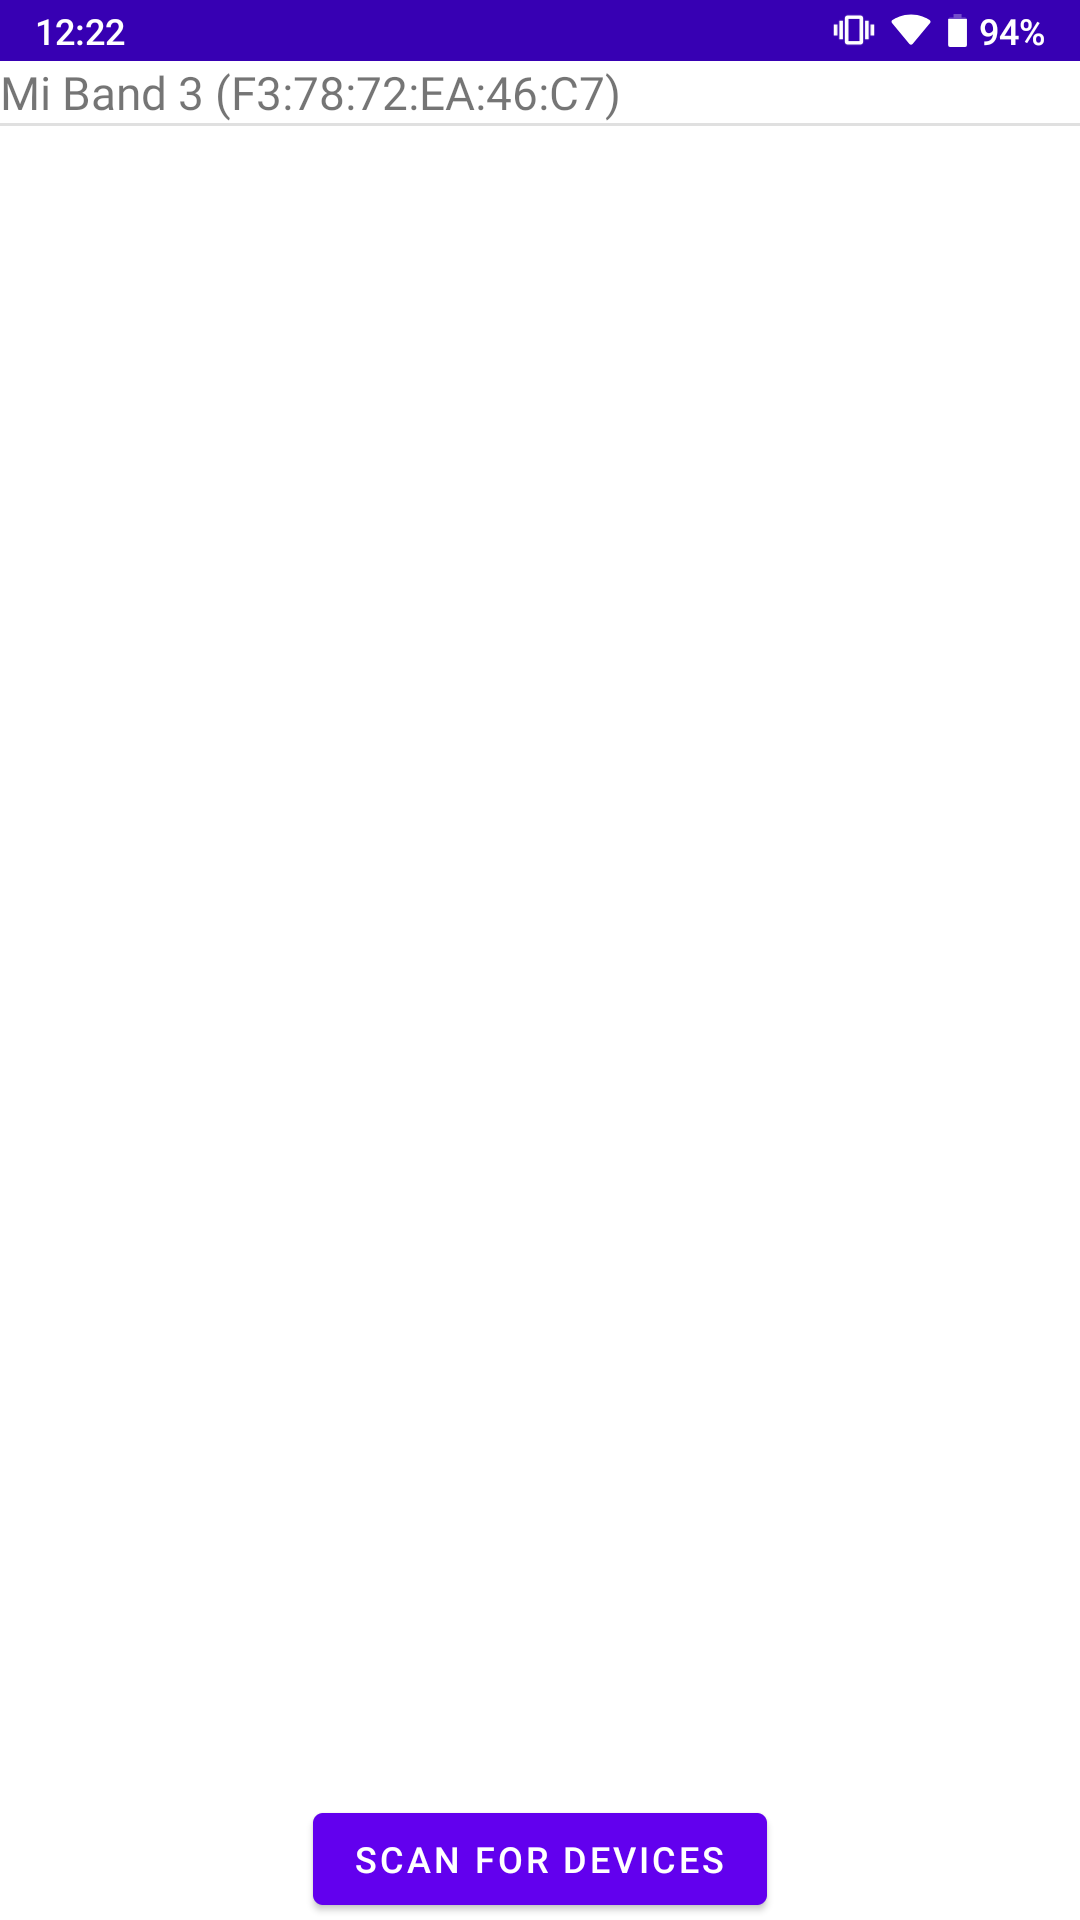
\includegraphics[width=0.27\textwidth]{app_screenshots/after_scan.png}}
    \end{center}
    \caption{{\color{dgray}Lista znalezionych w czasie skanu opasek MiBand 3.}} \label{afterScan}
\end{figure}
\begin{figure}[H]
    \begin{center}
        \setlength{\fboxsep}{0pt}%
        \setlength{\fboxrule}{0.3pt}%
        \fbox{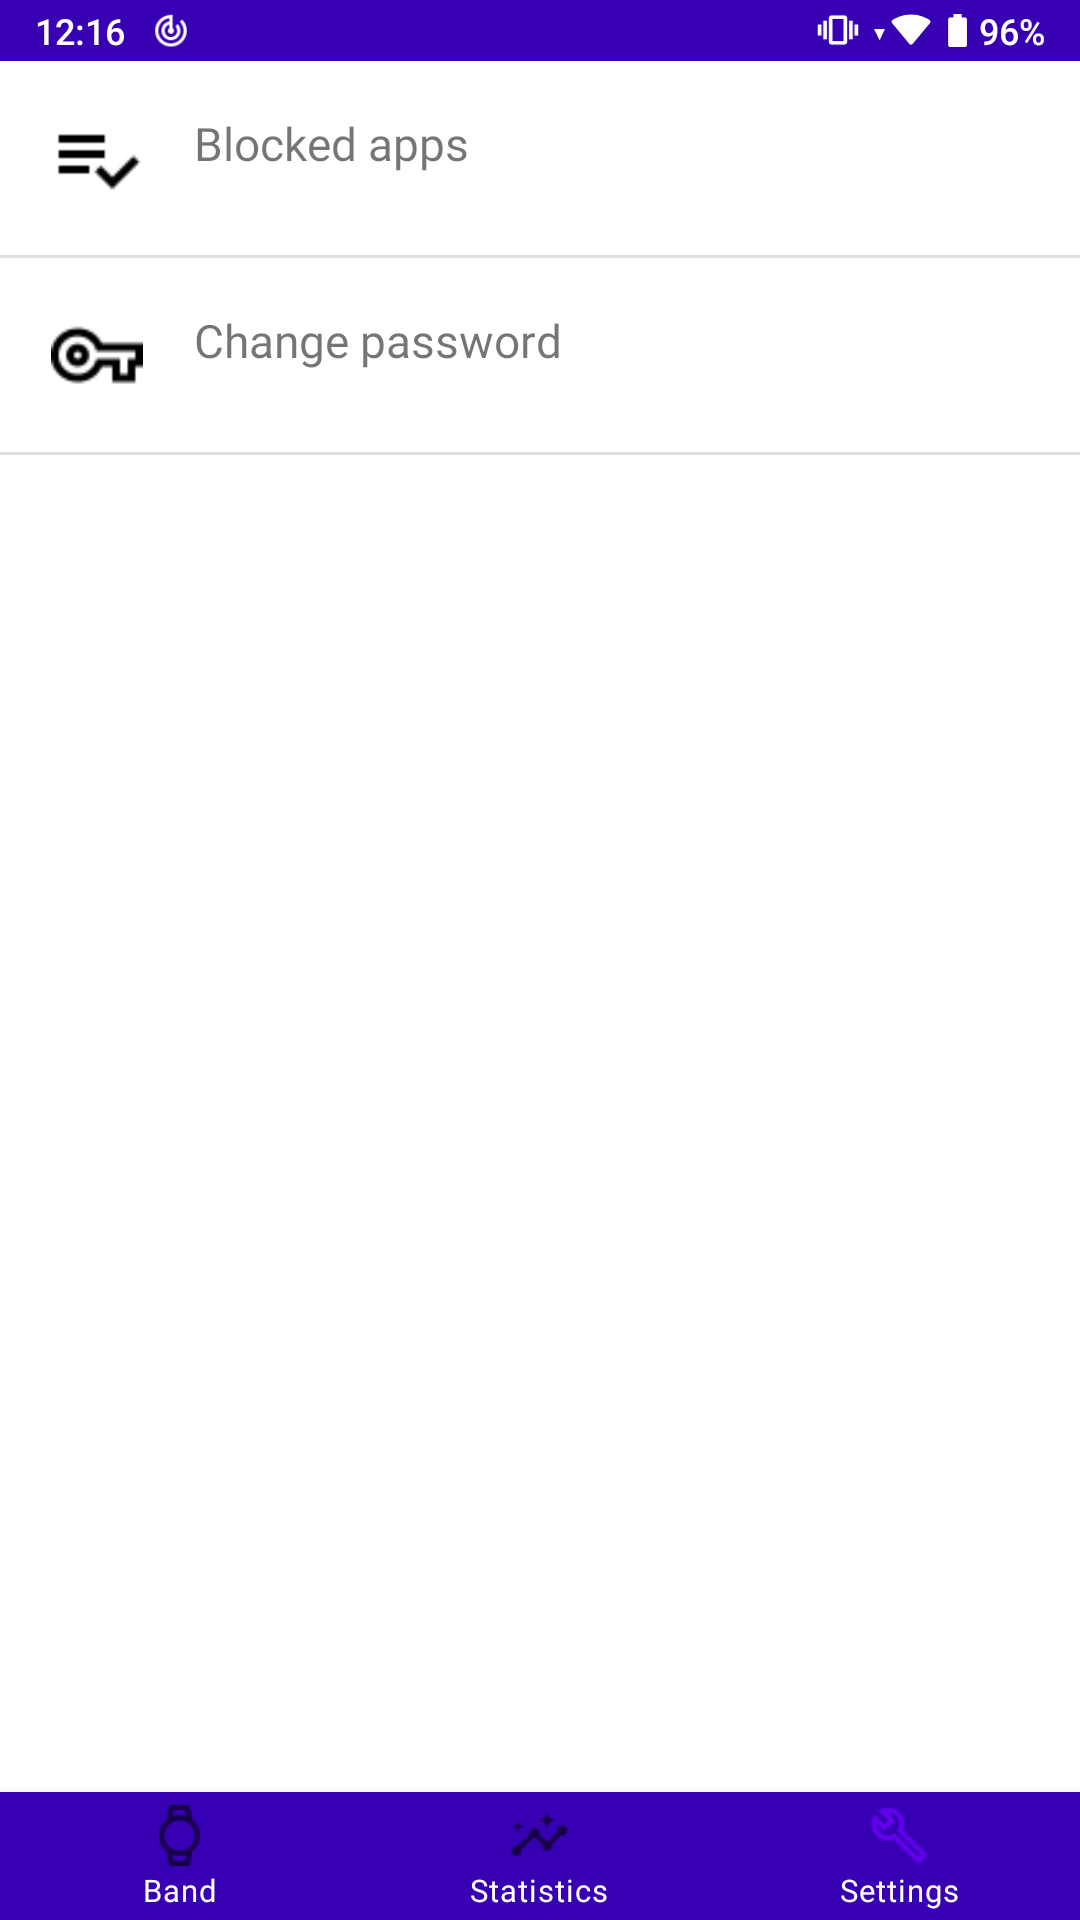
\includegraphics[width=0.27\textwidth]{app_screenshots/settings_screen.png}}
    \end{center}
    \caption{{\color{dgray}Ustawienia aplikacji.}} \label{Settings}
\end{figure}

\section{Przykłady użycia}
W tej sekcji przedstawię jak działa aplikacja od strony użytkownika poprzez opis czynności potrzebnych do wykonania określonych zadań, np. sprawdzenie stanu opaski, zmiana blokowanych aplikacji czy sprawdzenie statystyk.
\subsection{Wybór aplikacji do zablokowania}
Aby system zapewniał należytą ochronę musi wiedzieć, co jest chronione. W tym celu należy wybrać z listy zainstalowanych aplikacji, te które będą blokowane. Do listy tej można przejść z poziomu panelu ustawień \ref{Settings}, wybierając opcję \textit{Blocked apps}. Po naciśnięciu wyświetli się lista wszystkich aplikacji znajdujących się na telefonie. Aby objąć ochroną aplikację należy wykorzystać znajdujący się przy niej przełącznik. Kiedy ma kolor niebieski, aplikacja przy próbie uruchomienia w trakcie blokady będzie przeniosić użytkownika do formularza wprowadzania hasła \ref{enterPassword}.
\begin{figure}[H]
    \begin{center}
        \setlength{\fboxsep}{0pt}%
        \setlength{\fboxrule}{0.3pt}%
        \fbox{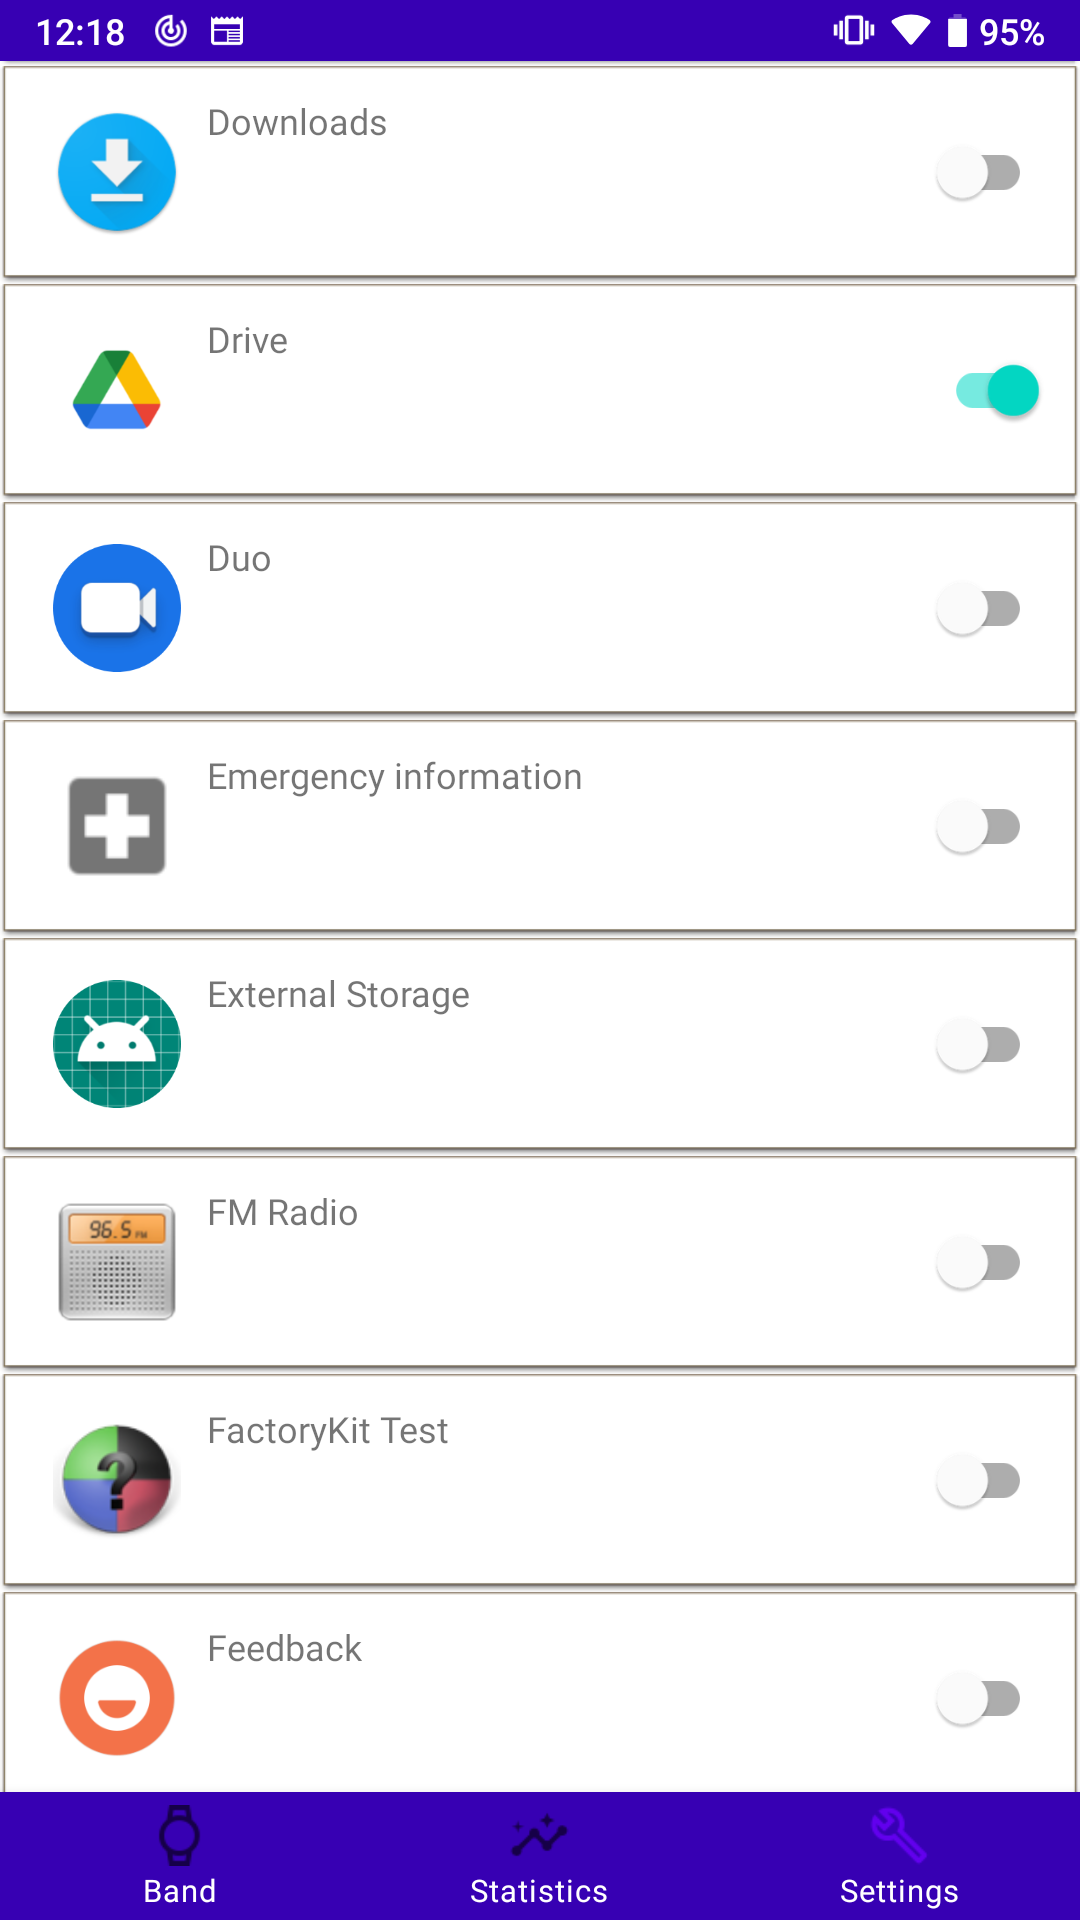
\includegraphics[width=0.27\textwidth]{app_screenshots/list_of_apps.png}}
    \end{center}
    \caption{{\color{dgray}Panel wyboru chronionych aplikacji.}} \label{appList}
\end{figure}
\subsection{Zmiana hasła użytkownika}
W przypadku, gdy użytkownik chce zmienić hasło wykorzystywane do dezaktywacji blokady, należy udać się do panelu ustawień \ref{Settings} i wybrać opcję \textit{Change password}. Po naciśnięciu pojawi się formularz zmiany hasła, gdzie należy wprowadzić stare hasło oraz dwa razy nowe hasło. Aby zapisać zmiany trzeba wcisnąć przycisk poniżej pól tekstowych.
\begin{figure}[H]
    \begin{center}
        \setlength{\fboxsep}{0pt}%
        \setlength{\fboxrule}{0.3pt}%
        \fbox{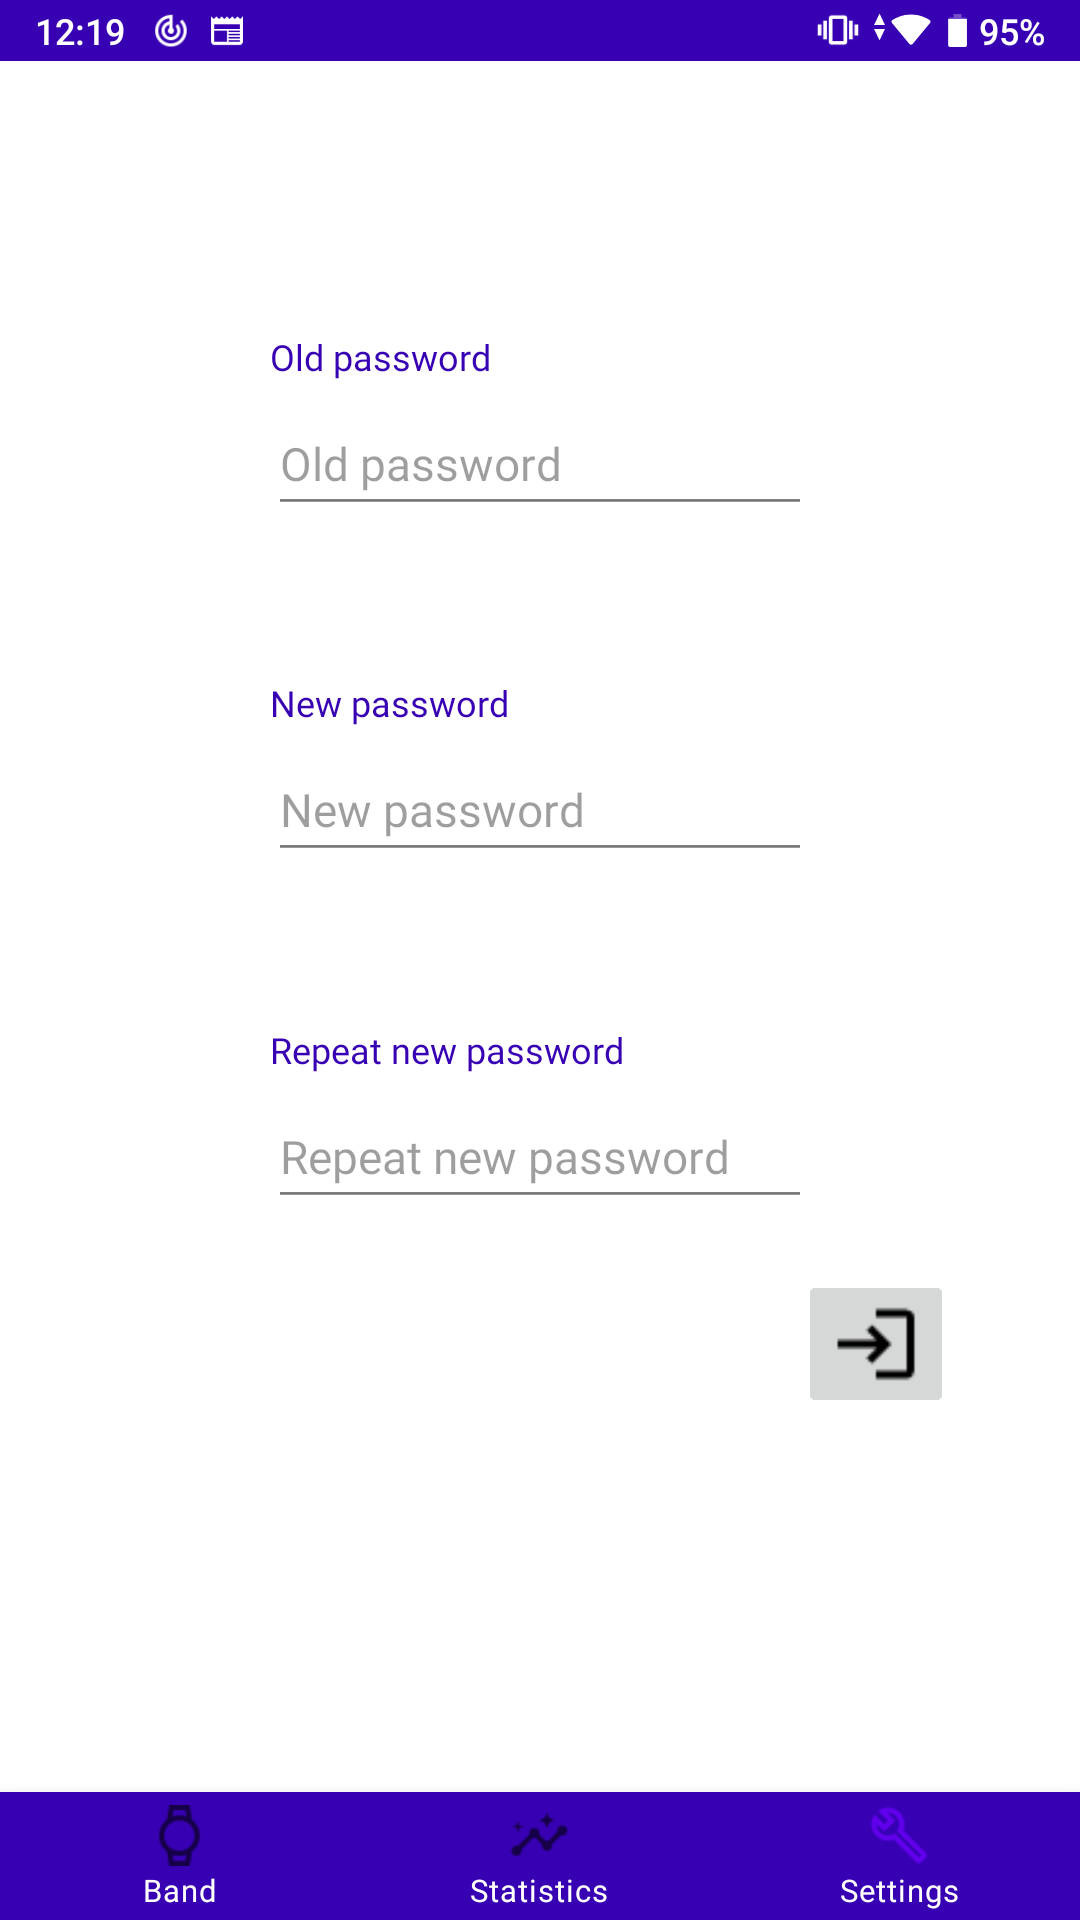
\includegraphics[width=0.27\textwidth]{app_screenshots/change_password.png}}
    \end{center}
    \caption{{\color{dgray}Panel zmiany hasła.}} \label{changePassword}
\end{figure}
\subsection{Wyświetlenie statystyk aktywności}
Aplikacja dostarcza użytkownikowi widok, w którym podane są informacje na temat zarejestrowanych danego dnia kroków oraz ostatnia wartość pomiaru pulsu. Aby zobaczyć te dane należy uruchomić aplikację oraz wybrać z dolnego menu pozycję \textit{Statistics}.
\begin{figure}[H]
    \begin{center}
        \setlength{\fboxsep}{0pt}%
        \setlength{\fboxrule}{0.3pt}%
        \fbox{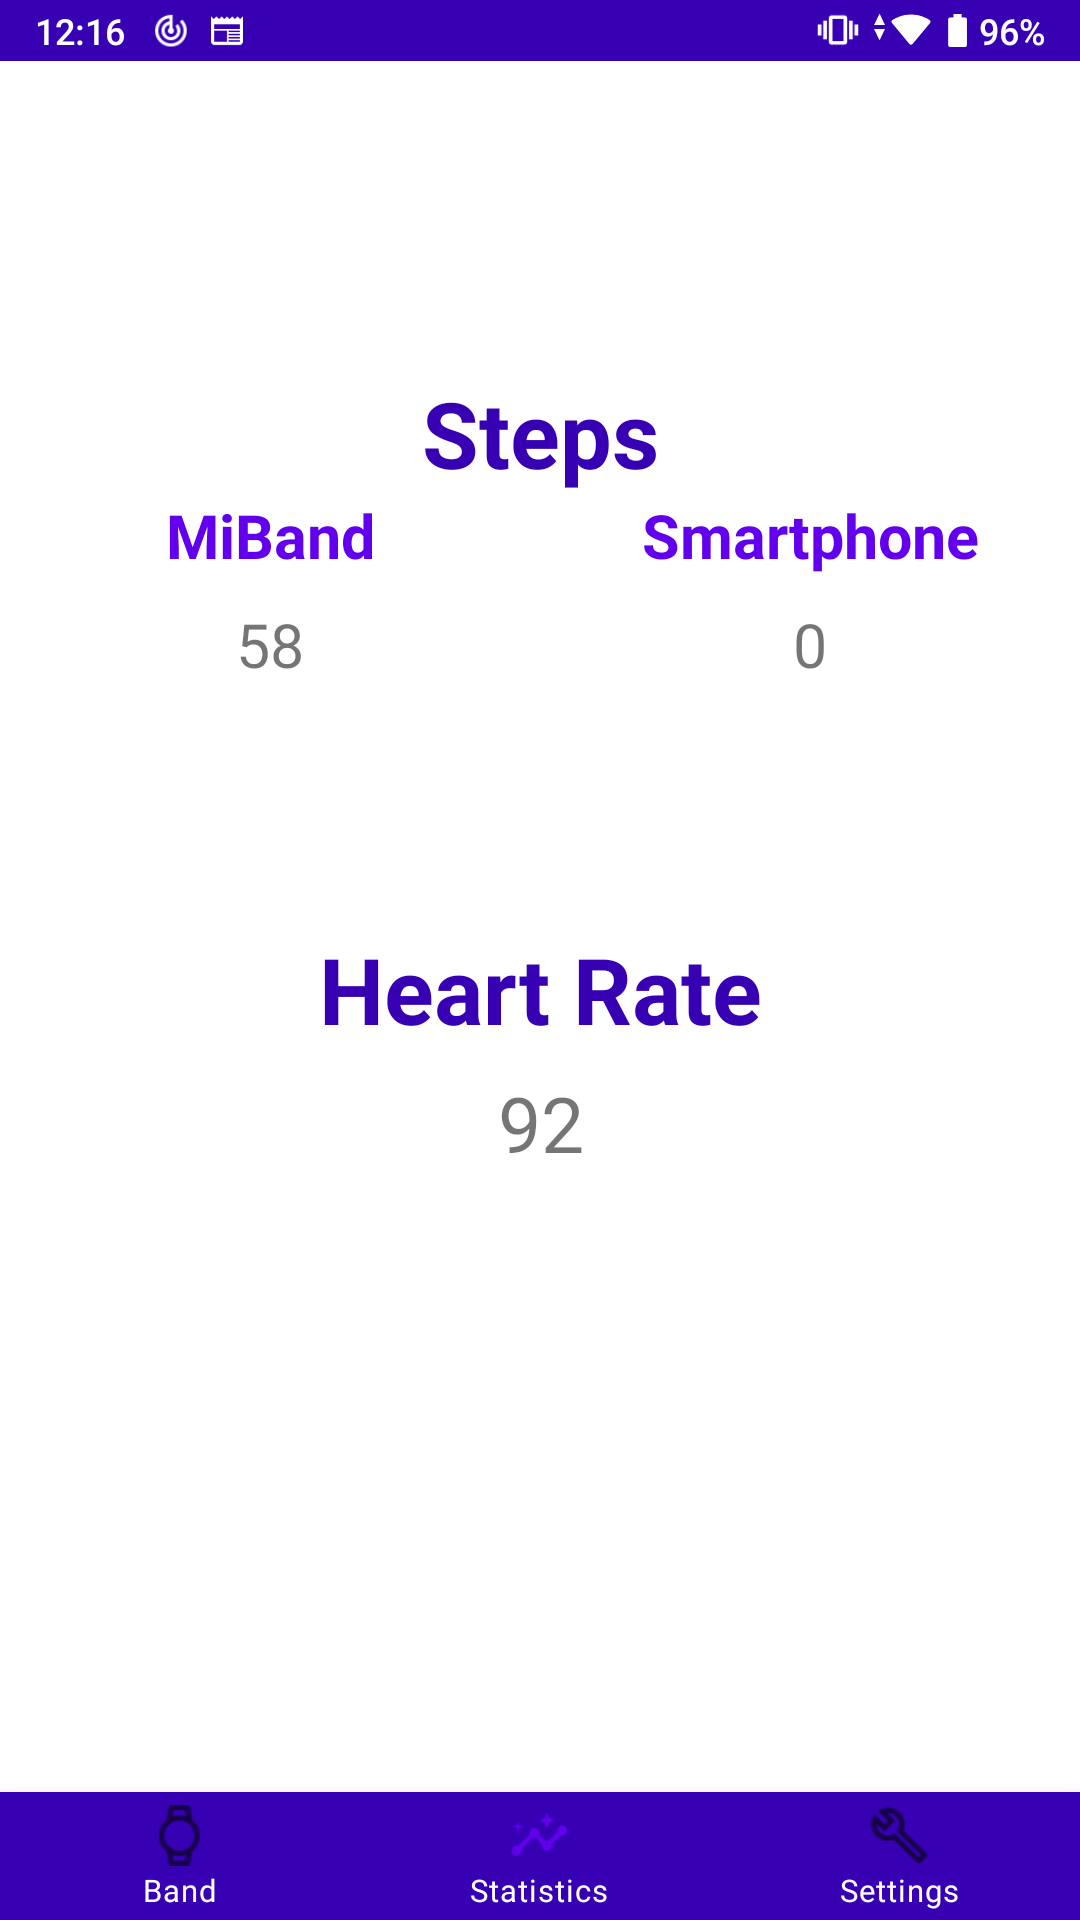
\includegraphics[width=0.27\textwidth]{app_screenshots/activity_stats.png}}
    \end{center}
    \caption{{\color{dgray}Panel informujący o ostatnich zarejestrowanych aktywnościach.}} \label{Stats}
\end{figure}
\subsection{Wyświetlenie informacji o opasce}
Aplikacja zapewnia także panel, w którym można sprawdzić podstawowe informacje o opasce oraz jej stan baterii. Aby uruchomić ten panel należy wejść do głównego widoku aplikacji i wybrać z menu dolnego pozycję \textit{Band}.
\begin{figure}[H]
    \begin{center}
        \setlength{\fboxsep}{0pt}%
        \setlength{\fboxrule}{0.3pt}%
        \fbox{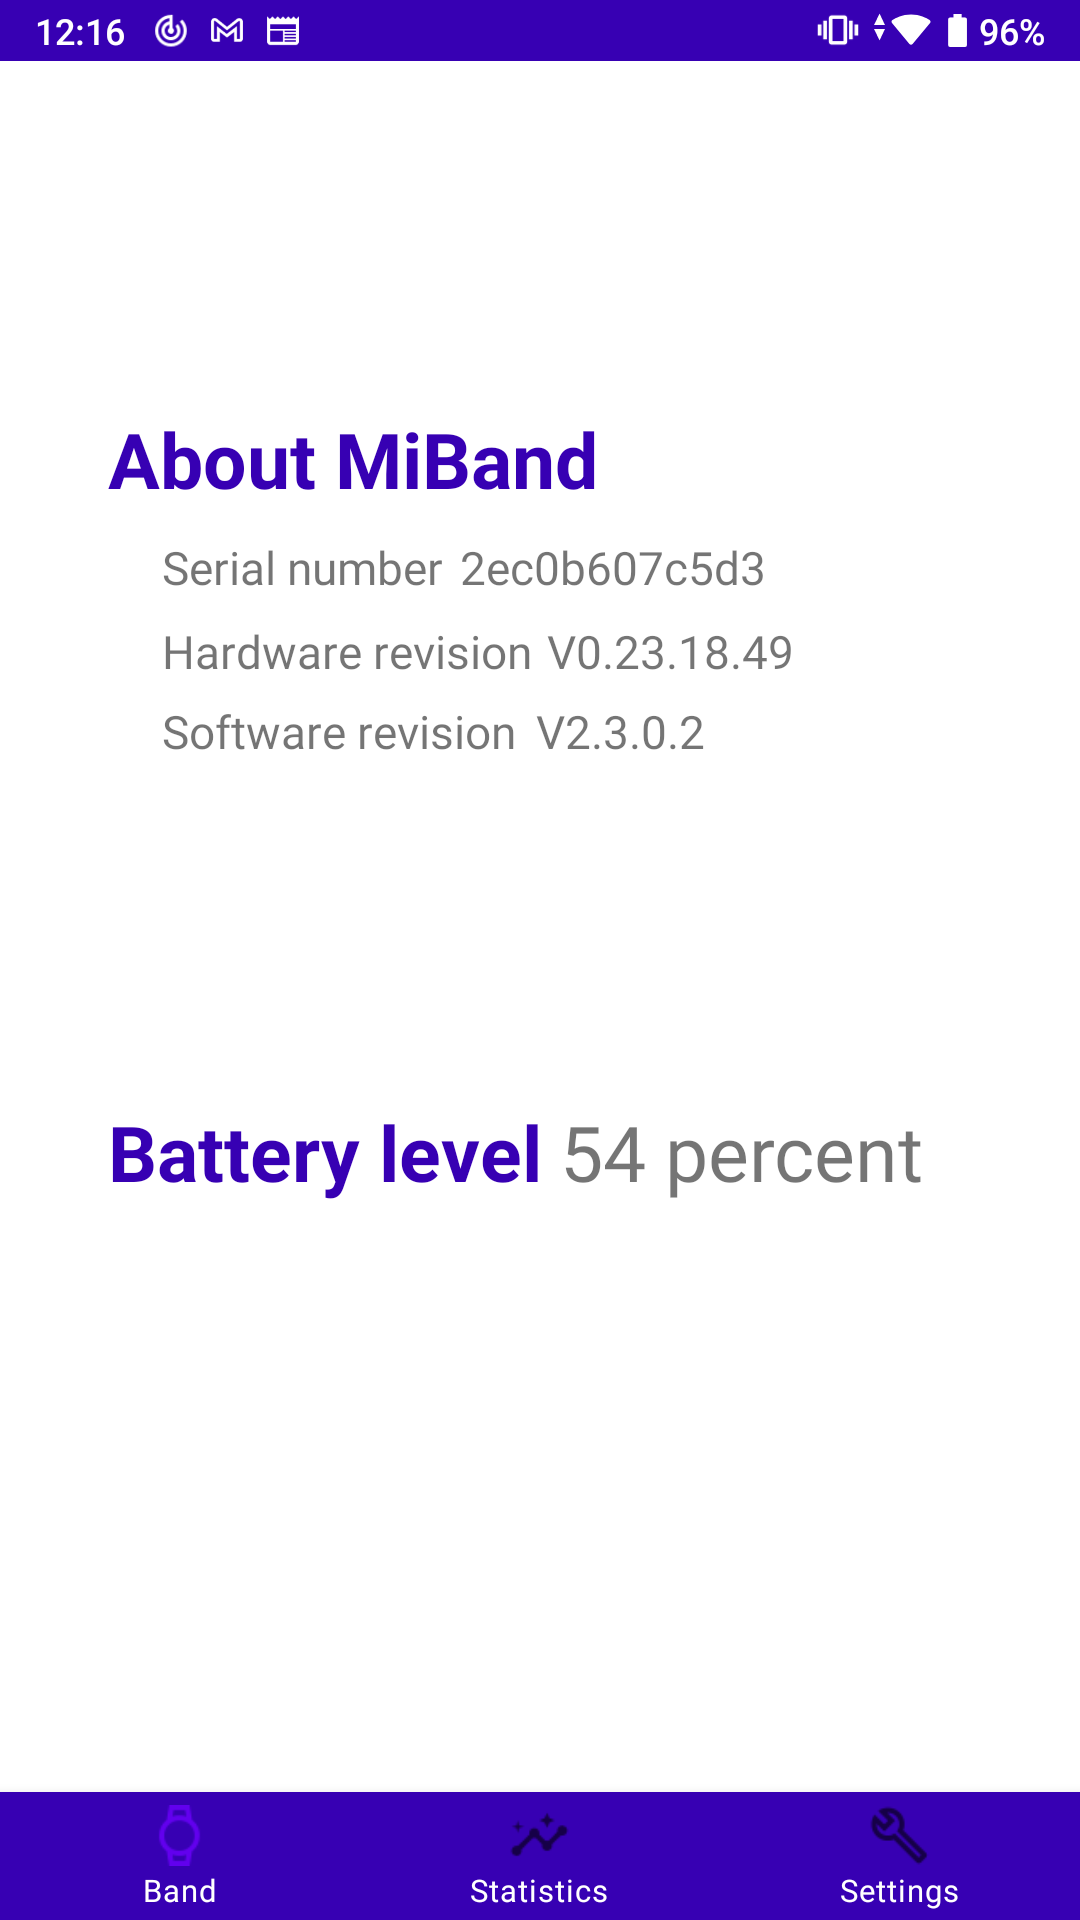
\includegraphics[width=0.27\textwidth]{app_screenshots/band_info.png}}
    \end{center}
    \caption{{\color{dgray}Panel informujący o stanie opaski.}} \label{BandInfo}
\end{figure}
\subsection{Odblokowanie systemu}
Wyłączenie aktywnej blokady odbywa się w na kilka sposobów. Użytkownik może:
\begin{itemize}
    \item nacisnąć powiadomienie o blokadzie;
    \item uruchomić aplikację;
    \item lub podjąć próbę uruchomienia jednej z chronionych aplikacji.
\end{itemize}

W każdy z tych przypadków system przekieruje użytkownika do formularza wprowadzania hasła. Po wpisaniu poprawnej wartości oraz zatwierdzeniu jej blokada zostaje zdjęta, a następnie uruchamiana jest usługa monitorująca aktywność.
\newline\newline\newline
\begin{figure}[H]
    \begin{center}
        \setlength{\fboxsep}{0pt}%
        \setlength{\fboxrule}{0.3pt}%
        \fbox{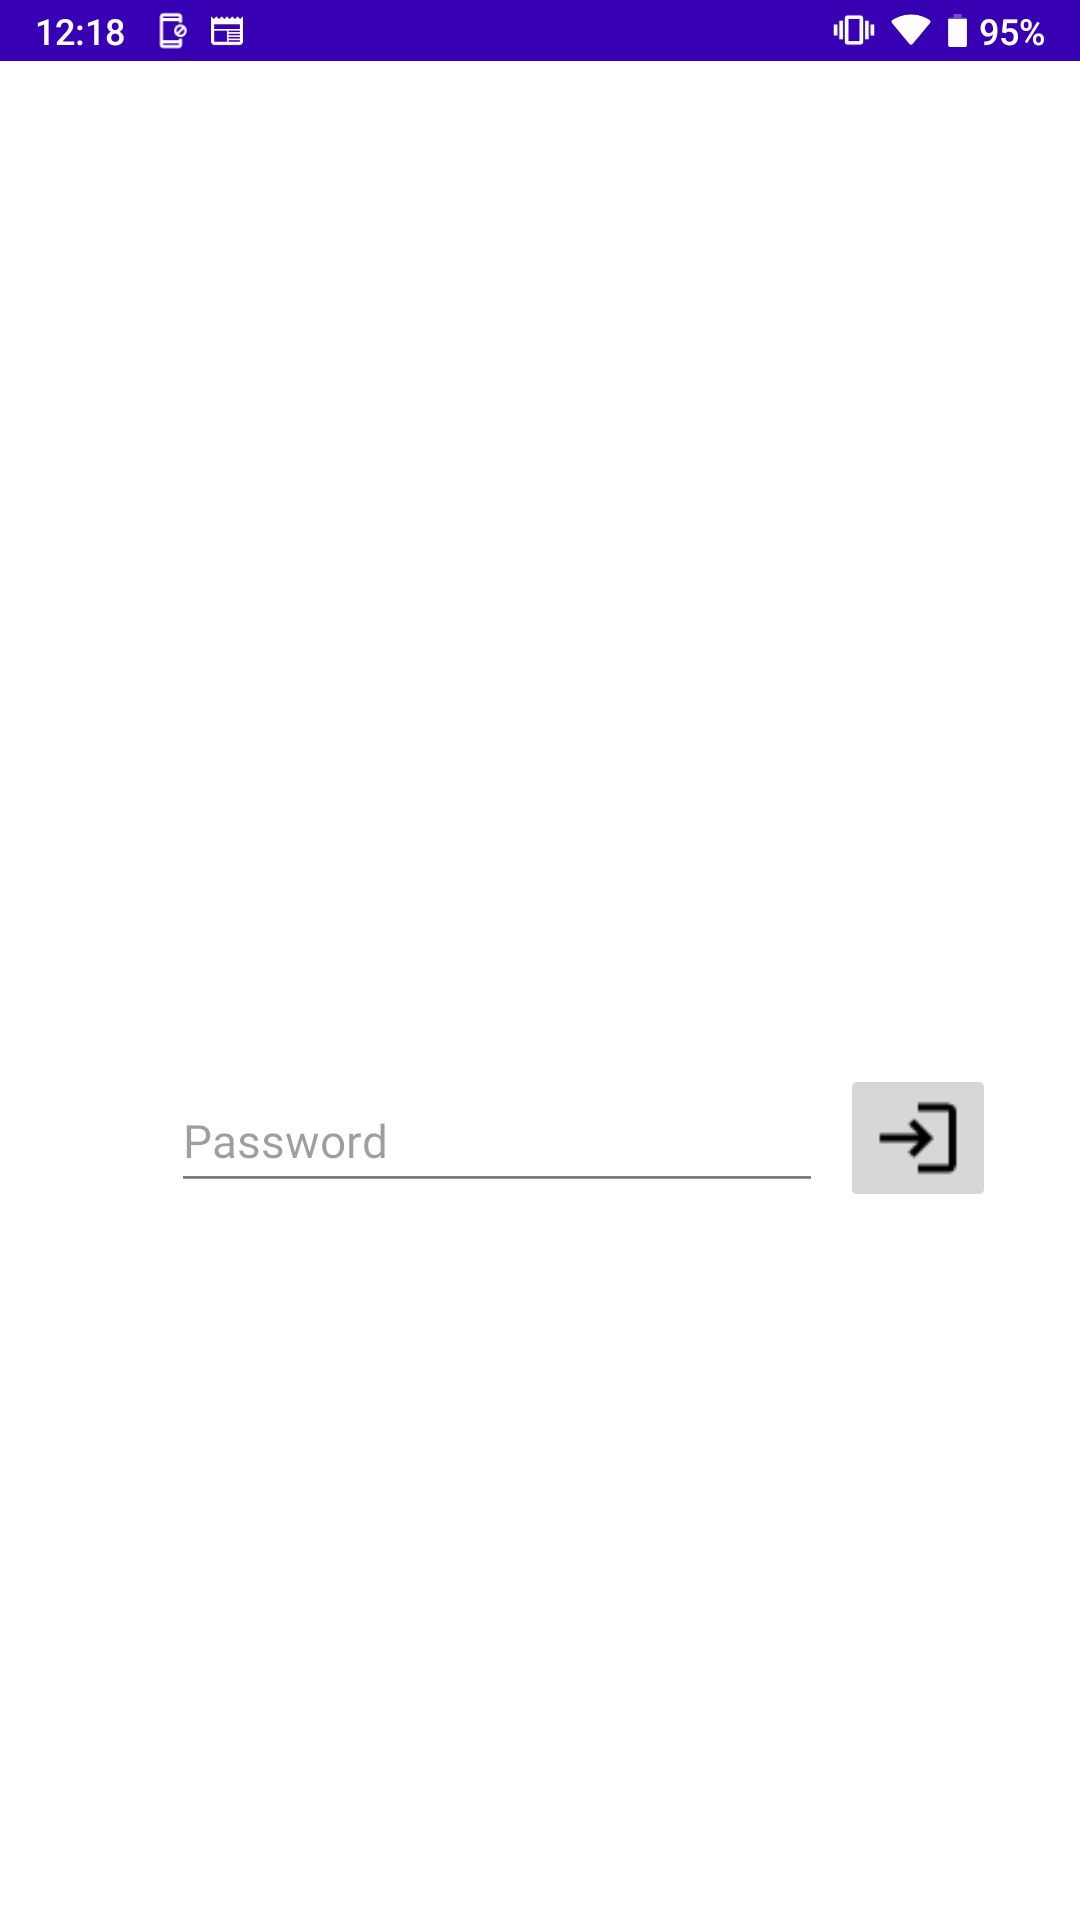
\includegraphics[width=0.27\textwidth]{app_screenshots/unblocking_activity.png}}
    \end{center}
    \caption{{\color{dgray}Formularz wprowadzania hasła.}} \label{enterPassword}
\end{figure}
	\cleardoublepage
	
	\chapter{Podsumowanie}
\thispagestyle{chapterBeginStyle}
W pracy dokonano analizy problemu wykorzystania fizycznych kluczy bezpieczeństwa w celu zabezpieczenia smartfonów oraz zapewnienia stałej autoryzacji dla systemu Android. Przedstawiono któtki opis proponowanego rozwiązania tego problemu. Następnie przedstawiono istniejące klucze działające z urządzeniami mobilnymi oraz rozwiązania pozwalające zabezpieczyć te urządzenia. Omówiono różnice między nimi a projektowanym systemem. W kolejnym rozdziale przedstawiono projekt aplikacji przy użyciu diagramów UML. W następnym rozdziale opisano wykorzystane do implementacji technologie. Zaprezentowano także szczegóły systemu blokującego dostęp do aplikacji. Opisano również wyczerpująco protokół komunikacji z opaską MiBand 3. Określono też sposoby analizy rejestrowanych danych o aktywności użytkownika. Na końcu przedstawiono instrukcję korzystania z aplikacji dla użytkownika wraz z wymaganiami sprzętowymi oraz procedurą instalacji. 
\section{Uzyskane wyniki}
W implementacji aplikacji udało się zrealizować wszystkie wymagania funkcjonalne postawione we wstępie pracy. Jest jednak wiele rzeczy, które wymagają usprawnienia zanim system będzie mógł zostać wykorzystany do prawdziwej ochrony smartfona. Główną luką bezpieczeństwa są ograniczenia sprzętowe. 
\newline\newline
\indent Opaska MiBand 3 posiada dość mało bezpieczny protokół parujący, gdyż wysyła klucz wykorzystywany później do autentykacji pakietem ATT. Kolejnym mankamentem jest prędkość rejestrowania zdarzeń przez opaskę. Zanim zostanie zarejestrowane zdarzenie zdjęcia opaski mija często kilka minut co sprawia, że jest to praktycznie bezużyteczna informacja. Pomiar akcji serca odbywa się w minimalnych  odstępach minutowych, co jest zbyt długim okresem, by szybko reagować na zmiany. 
\newline\newline
\indent Z kolei system Android wymaga do inwazyjnych czynności takich, jak zamykanie innych aplikacji, aplikacji podpisanej przez system. Utrudnia to bardzo projektowanie aplikacji, które mogłyby być dystrybuowane użytkownikom poprzez Sklep Play. Dlatego w stworzonej aplikacji nie ma stuprocentowej możliwości zablokowania dostępu do innych aplikacji. Obecnie możliwe jest otworzenie stworzonej w pracy aplikacji, gdy zarejestrujemy obecność innej na pierwszym planie. Niestety aplikacje, które zostały wyrzucone z pierwszego planu wciąż są otwarte w tle. Nie można także prawdziwie zablokować wyłączenia formularza wprowadzania hasła, zważywszy na konieczność wykorzystania ekrenu dotykowego do wpisania hasła oraz to, że nawet wyłączenie dotyku nie pomogłoby w urządzeniach posiadających fizyczne przyciski nawigacyjne. Martwiąca jest także możliwość automatycznego zamknięcia działających w tle usług przez system Android. Zostały podjęte wszystkie kroki by temu zapobiec, wykorzystując usługi pierwszoplanowe oraz WakeLock ale minimalne ryzyko wciąż pozostaje. Ponowne uruchomienie aplikacji po restarcie urządzenia działa, lecz nie jest wystarczająco szybkie. W przeprowadzonych testach aplikacja uruchamiała się po kilku minutach od włączenia, co pozostawia wiele możliwości sabotażu systemu.
\section{Propozycje rozwoju}
W przyszłości aplikację można rozwinąć na następujące sposoby:
\begin{itemize}
    \item Wyłączyć łączność WiFi i dane komórkowe podczas aktywnej blokady. 
    \item Wdrożyć prawdziwe wyłączanie chronionych aplikacji podczas próby ich uruchomienia w czasie blokady.
    \item Dodać wsparcie dla większej ilości urządzeń typu smartband.
    \item Stworzyć dokładniejsze statystyki aktywności.
    \item Upodobnić aplikację do typowej aplikacji fitness, aby zamaskować ją w systemie.
    \item Dodać automatyczne usuwanie starych danych o aktywności.
    \item Uzupełnić algorytm blokowania o wykrywanie zdarzeń dodanych w systemie Android 10.
    \item Usprawnić szybkość wymiany danych ze smartbandem.
    \item Przeorganizować bazę danych na prawdziwie relacyjny model.
\end{itemize}







	\cleardoublepage
	
	
	%%%%%%%%%%%%%%%%%%%%%%%%%%%%%%%%%%%%%%%%%%%%%%%%%%%%%%%%%%%%%%%%%%%%%%%%%%%%%%
	%%%%%%%%%%%%%%%%%%%%%%%%%%%%%%% BIBLIOGRAFIA %%%%%%%%%%%%%%%%%%%%%%%%%%%%%%%%%
	%%%%%%%%%%%%%%%%%%%%%%%%%%%%%%%%%%%%%%%%%%%%%%%%%%%%%%%%%%%%%%%%%%%%%%%%%%%%%%

	\pagestyle{bibliographyStyle}
	\bibliographystyle{plabbrv}
	\bibliography{literatura}
	\thispagestyle{chapterBeginStyle}
        \addcontentsline{toc}{chapter}{Bibliografia}

	\cleardoublepage
	
	%%%%%%%%%%%%%%%%%%%%%%%%%%%%%%%%%%%%%%%%%%%%%%%%%%%%%%%%%%%%%%%%%%%%%%%%%%%%%%
	%%%%%%%%%%%%%%%%%%%%%%%%%%%%%%%%% DODATKI %%%%%%%%%%%%%%%%%%%%%%%%%%%%%%%%%%%%
	%%%%%%%%%%%%%%%%%%%%%%%%%%%%%%%%%%%%%%%%%%%%%%%%%%%%%%%%%%%%%%%%%%%%%%%%%%%%%%
	
	\appendix
	\pagestyle{appendixStyle}
	
	\chapter{Zawartość płyty CD}
\thispagestyle{chapterBeginStyle}
\label{plytaCD}

Płyta CD dołączona do pracy składa się z następujących elementów:
\begin{enumerate}
    \item Folder \textit{latex} zawierający kody źródłowe części pisemnej pracy dyplomowej w języku \LaTeX\, wraz z wykorzystywanymi grafikami.
    \item Folder \textit{lockband} zawierający kody źródłowe części implementacyjnej pracy dyplomowej w języku Kotlin wraz ze skompilowaną aplikacją mobilną na system Android w formacie APK. 
    \item Folder \textit{pdf} kryjący w sobie egzemplarz pracy dyplomowej w postaci pliku PDF.
\end{enumerate}



	\cleardoublepage

\end{document}

